% Options for packages loaded elsewhere
\PassOptionsToPackage{unicode}{hyperref}
\PassOptionsToPackage{hyphens}{url}
%
\documentclass[
]{report}
\usepackage{amsmath,amssymb}
\usepackage{lmodern}
\usepackage{iftex}
\ifPDFTeX
  \usepackage[T1]{fontenc}
  \usepackage[utf8]{inputenc}
  \usepackage{textcomp} % provide euro and other symbols
\else % if luatex or xetex
  \usepackage{unicode-math}
  \defaultfontfeatures{Scale=MatchLowercase}
  \defaultfontfeatures[\rmfamily]{Ligatures=TeX,Scale=1}
\fi
% Use upquote if available, for straight quotes in verbatim environments
\IfFileExists{upquote.sty}{\usepackage{upquote}}{}
\IfFileExists{microtype.sty}{% use microtype if available
  \usepackage[]{microtype}
  \UseMicrotypeSet[protrusion]{basicmath} % disable protrusion for tt fonts
}{}
\makeatletter
\@ifundefined{KOMAClassName}{% if non-KOMA class
  \IfFileExists{parskip.sty}{%
    \usepackage{parskip}
  }{% else
    \setlength{\parindent}{0pt}
    \setlength{\parskip}{6pt plus 2pt minus 1pt}}
}{% if KOMA class
  \KOMAoptions{parskip=half}}
\makeatother
\usepackage{xcolor}
\setlength{\emergencystretch}{3em} % prevent overfull lines
\providecommand{\tightlist}{%
  \setlength{\itemsep}{0pt}\setlength{\parskip}{0pt}}
\setcounter{secnumdepth}{-\maxdimen} % remove section numbering
\ifLuaTeX
  \usepackage{selnolig}  % disable illegal ligatures
\fi
\usepackage[]{natbib}
\bibliographystyle{plainnat}
\IfFileExists{bookmark.sty}{\usepackage{bookmark}}{\usepackage{hyperref}}
\IfFileExists{xurl.sty}{\usepackage{xurl}}{} % add URL line breaks if available
\urlstyle{same} % disable monospaced font for URLs
\hypersetup{
  hidelinks,
  pdfcreator={LaTeX via pandoc}}

\author{}
\date{}

\begin{document}

Title: PhD Thesis Author: R.L. Trotta

\markedchapter{Introduction}{Test Chapter}\label{Chapter-1}

\hypertarget{Section-1.1}{%
\section{Test}\label{Section-1.1}}

This is outlines how to setup each section.

\hypertarget{subsection-1}{%
\subsection{Subsection 1}\label{subsection-1}}

Some text\ldots{}

\hypertarget{subsection-2}{%
\subsection{Subsection 2}\label{subsection-2}}

Some more text\ldots{}

\hypertarget{subsubsection-1}{%
\subsubsection{Subsubsection 1}\label{subsubsection-1}}

The key is to have a space before and after each (sub)subsection.

\hypertarget{subsubsection-2}{%
\subsubsection{Subsubsection 2}\label{subsubsection-2}}

\begin{verbatim}
But make sure you don’t indent otherwise things will get weird. As you can see here it cuts it all off and can’t be read. Obviously, this is unwanted.
\end{verbatim}

\hypertarget{subsubsection-3}{%
\subsubsection{Subsubsection 3}\label{subsubsection-3}}

But here you can see that I did not indent and things don't get weird.
The lines no longer are cut off. I am not sure why this happens.
Begin\{verbatim\} is called whenever the indent is explicit in
Scrivener.

Also, add a space between paragraphs.
\markedchapter{Introduction}{Introduction}\label{Chapter-2}

\begin{quote}
\centering \emph{"To a man devoid of blinders, there is no finer sight than that of intelligence at grips with a reality that transcends it."}\\
\centering \emph{- Albert Camus, Myth of Sisyphus}
\end{quote}

\hfill

The meaning of life and existence has fascinated humanity for all of
written history. Starting with the foundations of mathematics and
philosophy by the ancient Greeks through the time of enlightenment, the
rationality driven by the materialistic world has shaped our current
society.~ \textless Describe the close relation of physics and
philosophy and how the two became so separated throughout the modern
era.\textgreater{}

Society in the 21st century is much different now. The modern era of
philosophy was~ coming to an end and a new era of post-modern
hyperreality started. (Dostoevsky said, ``if God is dead, then
everything is permitted'') Beginning~with Fredrick Nietzsche's famous
``God is dead'', the next 60 years was categorized years by a dichotomy
of profound scientific and unprecedented tragedy. Foundations of science
and society had been shattered and needed to be built anew. The theories
of general relativity and quantum mechanics rewrote the textbooks, just
as war unlike any ever seen were coming ahead. These two fronts collided
in the creation of nuclear weapons which provided countries with weapons
that hitherto been inconceivable.

The world changed forever in this moment. This was the moment where

\hypertarget{Section-2.1}{%
\section{Historical Context}\label{Section-2.1}}

\markedchapter{Theory}{Theory}\label{Chapter-3}

\hypertarget{Section-3.1}{%
\section{Quantum Chromodynamics}\label{Section-3.1}}

See section III.B on Medium energy nuclear physics (page 10):
{[}https://arxiv.org/pdf/2112.02309.pdf{]}.

The relevant part is the description of the correlation functions as
objects that need to be extracted from data. You may be able to use
something along the lines of this language to explain the PDF/GPDs in
your thesis.

\hypertarget{Section-3.2}{%
\section{Accessing Hadron Structure}\label{Section-3.2}}

\hypertarget{subsection}{%
\subsection{Subsection}\label{subsection}}

\hypertarget{subsubsection}{%
\subsubsection{Subsubsection}\label{subsubsection}}

\hypertarget{Section-3.3}{%
\section{Parton Distribution Functions and Form
Factors}\label{Section-3.3}}

\hypertarget{model-descriptions}{%
\subsection{Model Descriptions}\label{model-descriptions}}

\hypertarget{Section-3.4}{%
\section{Generalized Parton Distributions and Transverse Momentum
Distributions}\label{Section-3.4}}

Be brief on TMD section.

\hypertarget{model-descriptions-1}{%
\subsection{Model Descriptions}\label{model-descriptions-1}}

\hypertarget{Section-3.5}{%
\section{Experimental Considerations}\label{Section-3.5}}

Sullivan Process and Off-Shell Considerations

\hypertarget{Section-3.6}{%
\section{Kinematic Overview}\label{Section-3.6}}

Table of kinematics and purpose of each \(Q^2\) value (\(Q^2\), \(W\),
\(x\), \(t\)). Include phase space plots.
\markedchapter{Measurements at Jlab Hall C}{Measurements at Jlab Hall C}\label{Chapter-4}

\begin{minipage}[t]{0.2\textwidth}
    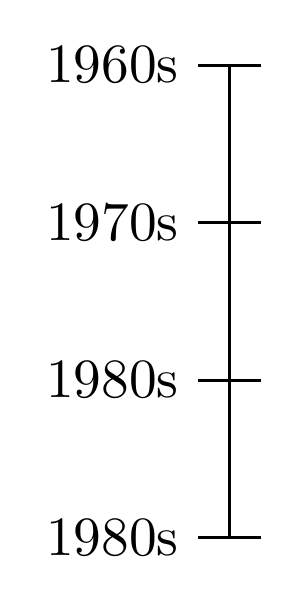
\begin{tikzpicture}[transform shape, scale=2]
        % Vertical line
        \draw[line width=1pt] (-1,0) -- (-1,3);
        % Horizontal lines and labels
        \foreach \y/\year in {0/1980s, 1/1980s, 2/1970s, 3/1960s} {
            \draw[line width=1pt] (-1.2,\y) -- (-0.8,\y);
            \node[anchor=east] at (-1.2,\y) {\year};
        }
    \end{tikzpicture}
\end{minipage}
\hfill
\begin{minipage}[t]{0.7\textwidth}
    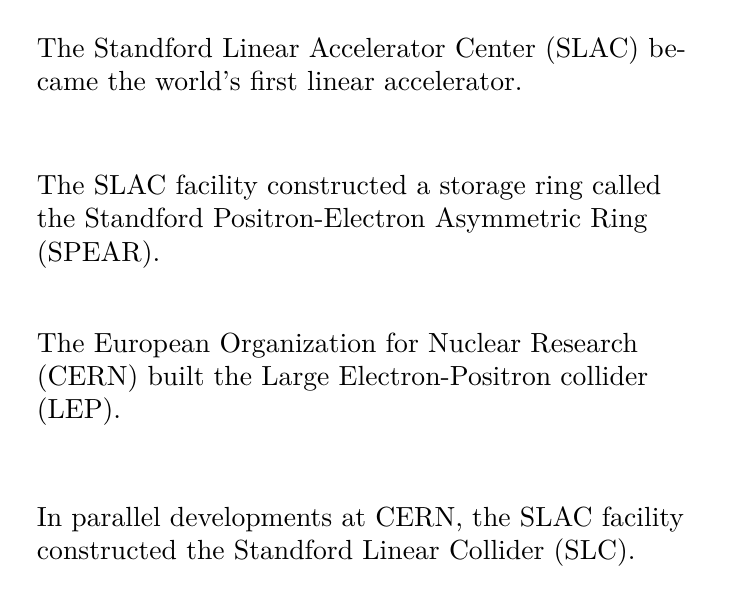
\begin{tikzpicture}[scale=2]
    \setstretch{1} % Set single spacing
        \node[align=left, text width=8.5cm] at (0,3.7) {\parbox{8.5cm}{The Standford Linear Accelerator Center (SLAC) became the world's first linear accelerator.}};
        \node[align=left, text width=8.5cm] at (0,2.7) {\parbox{8.5cm}{The SLAC facility constructed a storage ring called the Standford Positron-Electron Asymmetric Ring (SPEAR).}};
        \node[align=left, text width=8.5cm] at (0,1.7) {\parbox{8.5cm}{The European Organization for Nuclear Research (CERN) built the Large Electron-Positron collider (LEP).}};
        \node[align=left, text width=8.5cm] at (0,0.7) {\parbox{8.5cm}{In parallel developments at CERN, the SLAC facility constructed the Standford Linear Collider (SLC).}};
    \end{tikzpicture}
\end{minipage}

Above is a rough timeline of the accelerators and colliders that lead to
the eventual construction of the Continuous Wave Electron Accelerator
Facility (CEBAF) \cite{cahn_experimental_1989}. In the early 1990s, the
Continuous Wave Electron Accelerator Facility (CEBAF) was completed and
subsequently named Thomas Jefferson National Accelerator Facility
(Jlab), operated by SURA/PAE Applied Technologies for the U.S.
Department of Energy. In the 2000s, an upgrade to the CEBAF's 6 GeV
accelerator was approved and commissioning experiments began in the
Spring of 2018. The KaonLT (E12-09-011) experiment was performed in Hall
C at Jlab, running from September to December of 2018, with three weeks
off for the SIDIS experiments (E12-09-002 and E12-09-017), and
continuing from March to April of 2019.

\hypertarget{Section-4.1}{%
\section{Accelerator}\label{Section-4.1}}

Since 1995, the CEBAF at Jlab has been cornerstone to medium energy
nuclear research. CEBAF uses a high intensity continuous wave (CW) beam
to deliver electrons to four experimental halls (Halls A, B, C, and D).
In reality, this CW beam is not truly continuous, rather contains an
intrinsic microstructure of \textasciitilde2 ps short beam pulses that
occur at a fundamental frequency (\(f_0\)) of 1497 MHz
\cite{reece_continuous_2016}. This is a result of the Radio-Frequency
(RF) power used in the SRF resonant cavities which allows for four
sequential electron bunches that are subsequently sent to the four
halls.

\begin{Mfigure}{Schematic of CEBAF 12 GeV Upgrade}
  \centering
  \includegraphics[width=0.75\linewidth]{cebaf_12gev.pdf}
  \caption{Schematic of CEBAF 12 GeV Upgrade \cite{pilat_12_2012}.}
  \label{fig:2-1_cebaf12gev}
\end{Mfigure}



Each electron bunch is sent into the injector beamline, where they are
accelerated anywhere between 67 to 123 MeV, depending on the desired
beam energy \cite{pilat_12_2012}. From here, they are sent to the north
linac where they are accelerated further by 1.1 GeV. The beam is then
steered by the east arc into the south linac where they gain an
additional 1.1 GeV. Finally, the beam is steered back to the north linac
by the west arc where it can repeat this cycle. The beam can be
recirculated up to a total of five times, where each recirculation is
known as a pass. These passes correspond to the following beam energies:
1-pass (2.2 GeV), 2-pass (4.4 GeV), 3-pass (6.6 GeV), 4-pass (8.8 GeV),
5-pass (12.1 GeV).

Once the desired beam energy is obtained, it can be diverted to the
halls by using separators which are located at the end of the south
linac. In the 6 GeV era, a photo-cathode electron gun used three lasers
pulsing at 500 MHz (i.e.~\(f_0\)/3) which were eventually separated and
directed to each respective hall \cite{kazimi_operational_2019}. After
the 12 GeV upgrade, which includes the addition of Hall D, there had to
be a new beam pattern constructed in order to allow simultaneous beam in
all four halls. This new pattern included modifications to the injector
system and the RF separator extraction system. The injector system added
a fourth laser as well as a new 250 MHz pulse rate while the RF
extraction system had less straightforward changes as a pass-dependent
fix was implemented. For lower passes and when only Halls A, B, C are at
the highest passes, the laser pulses remained at 500 MHz. In the
situation where all four halls are running at the highest pass
(i.e.~5-pass), they are operating at 250 MHz. To allow this a new
separator called the ``5th pass separator'', was added which operates at
750 MHz. This ``5th pass separator'' (see figure
\ref{fig:2-1_cebaf12gev}) sends the separated beam around the 10th west
arc to Hall D.

\hypertarget{Section-4.2}{%
\section{Hall C Beam Line}\label{Section-4.2}}

Halls C accepts the beam through a long pipe that starts at the Beam
Switch Yard (BSY) and ends at the transport line
\cite{sta_jeerson_2019}. In order to reach the hall, the beam is bent in
the Hall C arc (see figure \ref{fig:2-2_hallc_arc}) using a series of
eight dipole magnets. From there, it enters the Hall C alcove where it
passes the Compton and \(\text{M\o{}ller}\) polarimeters to check the
polarity of the beam. At this point, the beam has entered the hall where
it will travel to the scattering chamber and, any beam not incidented
off the target, will end its journey in the beam dump.

\begin{Mfigure}{Hall C Arc to Beamline}
  \centering
  \includegraphics[width=0.75\linewidth]{hallc_arc.pdf}
  \caption{The Hall C arc which steers the beam to the beamline. Electron synchrotron radiation loss is shown with the yellow arrows.}
  \label{fig:2-2_hallc_arc}
\end{Mfigure}



Along this path, there are several beam diagnostic components that track
and monitor various aspects of the beam. The harps, Beam Position
Monitors (BPMs), and Beam Current Monitors (BCMs) are the primary
components used for diagnostics.

\begin{Mfigure}{Hall C Beamline}
  \centering
  \includegraphics[width=0.75\linewidth]{beamline.pdf}
  \caption{Hall C beamline from entrance of hall to the target scattering chamber.}
  \label{fig:2-2_beamline}
\end{Mfigure}



\hypertarget{beam-energy-measurement}{%
\subsection{Beam Energy Measurement}\label{beam-energy-measurement}}

The beam energy is determined by measuring the deflection of the
electron beam when it traverses through a known magnetic field in the
hall arc (see figure \ref{fig:2-2_hallc_arc}). In essence, the beam
energy is found by using the hall arc as a spectrometer
\cite{yan_beam_1993}. Using the basic description of a magnetic force
acting on an electron

\begin{equation} 
  |\vec{F_{B}}|=e|\vec{v_e}\times\vec{B}|=ev_{e}B_{\perp}=\frac{\gamma m_{e}v^2_e}{r_c}
  \label{eq:magnetic_force} 
\end{equation}

where \(e\) is the elementary charge , \(v_e\) is the electron velocity,
\(B_{\perp}\) is the magnetic field perpendicular to the velocity,
\(r_c\) is the radius of curvature, and \(\gamma\equiv(1-v^2_e/c^2)\).
Then using \(p_e=\gamma m_e v_e\) and \(r_c=dl/d\theta\), eq.
\ref{eq:magnetic_force} can be rewritten in terms of the electron
momentum

\begin{equation} 
  p_e=\frac{e}{\theta_{arc}}\int B dl
  \label{eq:electron_momentum} 
\end{equation}

where \(\theta_{arc}\) is the arc bend angle and \(dl\) is the
infintesimal arc length. Previous survey determined that the
\(\theta_{arc}\) was 34.3\(\degree\) and \(\int B dl\) is found by
mapping the magnetic fields of the arc dipoles at their corresponding
currents. The beam position and profile are measured superharps (see the
following sections) located at the entrance, middle, and exit of the
hall arc \cite{yan_superharp_1995}. Together there is an achievable
precision of \(\frac{\delta p}{p}\approx 5\times 10^{-4}\).

\hypertarget{beam-position-monitors-bpms}{%
\subsection{Beam Position Monitors
(BPMs)}\label{beam-position-monitors-bpms}}

The beam position and direction on the target is determined by three
BPMs, which can be found in on figure \ref{fig:2-2_beamline_components}.
Due to fringe fields of the SHMS magnets that arise from small forward
angle configurations, there are also two large diameter BPMs (known as
Big BPMs, see figure \ref{fig:2-2_beamline_bigbpms}). These BPMs are
cylindrical cavities consisting of a 4-wire antenna array which, to
minimizes synchrotron radiative damage, are rotated 45\(\degree\) with
respect to the horizontal and vertical axes. This array is made of thin
open ended wire striplines, used for RF signals requiring isolation from
surrounding circuitry, and tuned to \(f_0\). The beam induces an RF
signal in the antannae which is then either processed by the
Analog-to-Digital Converters (ADCs) or interpreted by the Experimental
Physics and Industrial Control System (EPICS).

\begin{Mfigure}{Hall C Beamline Components}
  \centering
  \includegraphics[width=0.75\linewidth]{beamline_components.pdf}
  \caption{The Hall C beamline components from entrance of hall to the target scattering chamber. The relevant distances from the scattering chamber are labeled.}
  \label{fig:2-2_beamline_components}
\end{Mfigure}



The BPMs can be read in by either of the two datastreams: EPICS or CODA.
The EPICS store the averaged position over 0.3 seconds while the
event-by-event information (i.e.~what is the processed by the ADC) is
stored by CODA. The raw beam postions from EPICS were used for this
experiment because of their simplicity
\footnote{The BPMS could have just as well been extracted from CODA, but this requires a separate calculation to convert the raw ADC to raw beam position values.}.
Once the raw beam values are obtained, the Hall C analysis software
(i.e.~calibrates relative to absolute beam position. The ratio of the
differences technique is used to determine the relative position of the
beam within 100 microns for currents above one \(\mu\)A. The superharps
(see next section) are calibrated with the BPMs to find the absolute
position.

\begin{Mfigure}{Hall C Beamline Big BPMS}
  \centering
  \includegraphics[width=0.75\linewidth]{beamline_bigbpms.pdf}
  \caption{Schematic of the Hall C beamline downstream, showing the Big BPMs (IPM3H08, IPM3H09) near the beam dump. [\cite{sta_jeerson_2019}]}
  \label{fig:2-2_beamline_bigbpms}
\end{Mfigure}



\hypertarget{harps}{%
\subsection{Harps}\label{harps}}

In order to obtain high precision measurements of the beam's profile and
position, the superharps are used. There are several superharps
throughout the beamline. There are two at the beginning and end of the
hall arc (see figure \ref{fig:2-2_hallc_arc}), one that is used by the
polarimeters (see figure \ref{fig:2-2_hallc_arc}), and the last two are
located just before the target (see figure
\ref{fig:2-2_beamline_components}).

Harps use a rotary encoder to determine absolute postion and three wires
connected to a fork to determine the profile. The superharp is attached
to a step motor where the linear movement is translated into rotary
motion. As the step motor moves, the encoder generates pulses equal to
the number of steps taken. This allows a relation between steps and beam
position which, along with the BPM information, is part of the
calibrations used in determining the absolute position. The step motor
movement also causes the wires the pass through the beam, where a signal
is generated in the form of a current produced by secondary electron
emission. This signal is amplified then sent to an ADC where the beam
profile can be obtained by fitting the spectrum. Since the harp moves
through the unrastered (see next section) beam, these ``harp scans'' are
done as an initial procedure when beam first becomes available.

\hypertarget{raster}{%
\subsection{Raster}\label{raster}}

The beam intensity can be so extreme that, after prolonged exposure,
there can be localized heating or damage to the target chamber or, even,
detectors. To prevent such damages, a raster is used to spread the beam
over a larger area, which, in turn, distributes the beam's power more
uniformly over the target. A raster applies small, controlled
oscillations, in both the horizontal and vertical directions, causing
the beam to scan back and forth or in a circular pattern, depending on
the desired beam profile. These oscillations are applied to the beam
steering elements, such as the magnets.

\begin{Mfigure}{XY Raster Plot}
  \centering
  \includegraphics[width=0.75\linewidth]{raster.pdf}
  \caption{Fast raster XY plot of run 6881 during 4.9 GeV. The uniform beam dispersion is evident by the teal homogeneity which corresponds to ~15 events per bin.}
  \label{fig:2-2_raster}
\end{Mfigure}



Hall C has three types of rasters available: \(\text{M\o{}ller}\), fast,
and slow. The \(\text{M\o{}ller}\) and slow rasters are used for special
circumstances. The fast raster is primarily used. It works by driving AC
current from a 250 W audio amplifier to horizontal and vertical air-core
magnets, creating a rectangular beam dispersion. A 2x2 m\(m^2\) fast
raster was used throughout the experiment.

\hypertarget{beam-current-monitors-bcms}{%
\subsection{Beam Current Monitors
(BCMs)}\label{beam-current-monitors-bcms}}

Beam current is measured using BCMs, which, in Hall C, take two primary
forms: Unser monitor or RF cavity. An Unser monitor, also known as a
Parametric Current Transformer (PCT), is a toroidial transformer that is
designed to be non-destructive and acts as the absolute reference frame
\cite{unser_parametric_1992}. The circular magnetic field of the toroid
magnetizes strips of permeable matrial as the beam passes through it,
this sends a current, proportional to the beam current, to a
compensating coil thus canceling out the field of the beam. RF cavities,
on the other-hand, are cylindrical, stainless steal cavities that work
off the basic ideas of a waveguide. When the beam passes through them at
their resonant frequency (i.e.~\(f_0\)), they are excited and an antenna
inside couples this power to a heliax cable to eventually be processed.

An Unser monitor and two RF cavities (BCM1 and BCM2) wrapped in thermal
blankets, for temperature stabilization, make up the primary current
monitoring system and are located upstream from the target. There is
also an additional three RF cavities (BCM4A, BCM4B, and BCM4C) enclosed
in a thermally stabilized box that are aviable if the beamline
configuration allows. These are located further upstream than the Unser
or BCM1, just inside the hall entrance. Finally, there is one last BCM
(BCM17) located upstream from the Compton polarimeter on the 3C17
girder. In addition to these BCMs, that are part of the Hall C current
measurement system, there is another BCM immediately upstrem of the
target which is used to monitor beam loss and is primarily there for
machine protection.

\begin{Mfigure}{BCM1/2 and Unser}
  \centering
  \includegraphics[width=0.75\linewidth]{bcm_unser.pdf}
  \captionsetup{width=0.95\textwidth} % Adjust the caption width here
  \caption{Drawing showing BCM1 and BCM2 on either side of the Unser monitor. A Unser wire calibration can be performed by passing a wire (labeled calibration wire), with an accurately known current, through the Unser monitor to measure the gain of the electronic chain. [\cite{sta_jeerson_2019}]}
  \label{fig:2-2_bcm_unser}
\end{Mfigure}



The signal for the Unser monitor drifts significantly over the course of
a few minutes, so it cannot be used as a continuous current monitor.
Still, being the absolute reference frame means that the Unser can be
used to calibrate the cavities which are used for continous current
monitoring. In order to correct for this drift, a ``Unser wire
calibration'' is performed, wherein, a wire, with a known current, is
run through the Unser and is used to measure the gain of the electronic
chain (see figure \ref{fig:2-2_bcm_unser}). This gain is then
calibrated, which corrects for the drift in the absolute frame. The
combination of the Unser monitor with BCM1 and BCM2 allows a beam
current with an absolute accuracy of about 1 \cite{denard_high_2001}.

\hypertarget{Section-4.3}{%
\section{Target}\label{Section-4.3}}

At the end of the beamline, the electron beam has finally reached the
target chamber. The target chamber was designed to isolate the beam line
vacuum from the rotating spectrometers. The chamber houses a loop of
cryogenic targets (see figure \ref{fig:2-3_target_loop}), such as liquid
hydrogen, as well as a variety of solid targets on the ladder, such as
Aluminum. Targets used during the E12-09-011 experiment can be seen in
table \ref{tab:2-3_target_loop}. Additional targets, used for other
experiments, were on the ladder, see Ref. \cite{sta_jeerson_2019} for
more details.

\begin{Mfigure}{Target Loop}
  \centering
  \includegraphics[width=0.75\linewidth]{target_loop.pdf}
  \caption{ CAD view of the cryogenic and solid target ladders \cite{sta_jeerson_2019}. There are three cyrogenic loops above the solid target ladder.}
  \label{fig:2-3_target_loop}
\end{Mfigure}



\begin{Mtable}{Target Loop}
  \centering
  \begin{tabular}{|c|c|c|c|}
    \hline
    \textbf{Loop Number} & \textbf{Target} & \textbf{Length} & \textbf{Current Limits} \\
    \hline
    1 & $^{2}\mathrm{He}$ & 4 cm & - \\
    1 & $^{2}\mathrm{He}$ & 10 cm & - \\
    2 & L$H_2$ & 10 cm & - \\
    3 & L$D_2$ & 10 cm & - \\
    - & Dummy + C & 10 cm & - \\
    - & Dummy & 10 cm  & - \\
    - & Dummy & 4 cm  & - \\
    - & Optics 1 & 20 cm  & - \\
    - & Optics 2 & -  & - \\
    - & Carbon Hole & -  & - \\
    - & Carbon 6\% A & -  & - \\
    - & Carbon 6\% B & -  & - \\
    - & Carbon 0.5\% & -  & - \\
    - & $B_4$C-10 & -  & - \\
    - & $B_4$C-11 & -  & - \\
    - & Be & -  & - \\
    - & Carbon 1.5\% & -  & - \\
    \hline
    \end{tabular}
  \caption{Break down of all targets available during the running period. The three cryogenic targets are labeled alongside their corresponding loops. The target length is also provided for each type.}
  \label{tab:2-3_target_loop}
\end{Mtable}



This experiment required a proton target so the primary one used was
liquid hydrogen (\(LH_2\)). The \(LH_2\) was contained in loop 2, while
the liquid Deuterium (\(LD_2\)) was in loop 3 and loop 3 was empty, only
containing \(^{2}\mathrm{He}\) gas to keep vacuum pressure. \(LH_2\) is
kept at a temperature of 19 \(\pm 0.1\) K(\textasciitilde25 psia) and
density of 0.07231 g/\(cm^3\) \cite{smith_g_hall_2016}. There needs to
be special care taken with all cryogenic targets as they have a strict
freezing and boiling points, therefore the temperatures need to be
closely monitored by the target operators to avoid disaster. For
\(LH_2\), the freezing and boiling point, respectively, are 13.8 K and
22.1 K.

The \(LH_2\) target may have been the main target used but it was not
the only one used. The 10 cm Aluminum Dummy target was also used
extensively. This solid target consists of aluminum foils mounted in
separate frame that correspond to the cryogenic entrance and exit
windows. This setup is purposeful as the 10 cm Aluminum Dummy target is
used for ``dummy subtractions'' which are the removal of background
events in the data associated with the aluminum frames that house the
cryogenic targets.

The the Carbon 1.5\% target was also used. Because these targets are
made of carbon, they withstand very high currents, which makes them
excellent for sieve and luminosity studies. These studies examine optics
and efficiencies, respectively, and will be discussed in more detail in
following sections and chapters.

Beyond these two targets used for data, there are also the Carbon Hole,
Optics-1 targets which are used for beam centering and spectrometer
optics, respectively. The Carbon Hole is a thin carbon foil that has
been cut so that there is a central 2 mm diameter hole. Similar to
figure \ref{fig:2-2_raster}, the rastered beam can be used to adjust the
beam to a more central position. With a Carbon Hole target, a rastered
XY plot will now have a hole showing the beam's central position. Shift
workers communicate adjustments to MCC so that it can be steered to its
proper position. The Optics-1 target is made of carbon foils located at
5 cm in front the entrance and 5 cm behind the exit cryogenic target
windows. These are used for spectrometer optics optimization studies,
which will be discussed in a following section.

\hypertarget{Section-4.4}{%
\section{Spectrometers}\label{Section-4.4}}

The distinctive feature of Hall C lies in its possession of two high
luminosity (\(10^{39}\text{cm}^{-2}\text{s}^{-1}\)) magnetic
spectrometers, namely the High Momentum Spectrometer (HMS) and the Super
High Momentum Spectrometer (SHMS). These cutting-edge instruments
empower physicists to conduct unparalleled precision in cross-section
experiments. Each spectrometer rests on rotatable support structures
that can move along rails, all while keeping the optical elements and
detectors aligned relative to the target.

\begin{Mtable}{Spectrometer Specifications}
  \centering
  \begin{tabular}{|c|c|c|c|}
    \hline
    \textbf{Parameter} & \textbf{HMS} & \textbf{SHMS}\\
    \hline
    Central Momentum & 0.4 - 7.4 GeV/c & 2 - 11 GeV/c \\
    Momentum Acceptance & $\pm$10\% & -10\% - +22\% \\
    Momentum Resolution & 0.1\% - 0.15\% & 0.03\% - 0.08\% \\
    Scattering Angle Range & 10.5$\degree$ - 90$\degree$ & 5.5$\degree$ - 40$\degree$ \\
    \hline
    Horizontal Angle Acceptance & $\pm$32 mrad & $\pm$18 mrad \\
    Horizontal Angle Resolution & 0.8 mrad & 0.5 - 1.2 mrad \\
    Vertical Angle Acceptance & $\pm$85 mrad & $\pm$50 mrad \\
    Vertical Angle Resolution & 1.0 mrad & 0.3 - 1.1 mrad \\
    Solid Angle Acceptance & 8.1 msr & >4 msr \\
    \hline
    Maximum Event Rate & 2000 Hz & 10,000 Hz \\
    e/h Discrimination & >1000:1 at 98\% efficiency & >1000:1 at 98\% efficiency \\
    $\pi$/K Discrimination & 100:1 at 95\% efficiency & 100:1 at 95\% efficiency \\
    \hline
  \end{tabular}
  \caption{Break down of the HMS and SHMS specifications and capablilities..}  
  \label{tab:2-4_spectrometer}
\end{Mtable}



A breakdown of the spectrometer specifications and capablilities are
given in table \ref{tab:2-4_spectrometer}. The sucess of the HMS at
hadron detection during the 6 GeV era inspired the SHMS. Because of
this, the two spectrometers are very similar in design. Inside their
heavily shielded detector hut, both consist of a series of dipoles and
quadrupoles followed by a lineup of particle detectors. The dipoles and
quadrupoles, together known as the optical elements, are used to steer
the scattered particles to the detectors from the target chamber. These
steered particles are then tracked through drift chambers (DC) by
reconstructing their trajectories from the focal plane back to the
target. These tracked particles are then identified through a series of
hodoscopes, Cerenkov detectors and calorimeters.

\begin{Mfigure}{Spectrometer Setup}
  \centering
  \includegraphics[width=0.75\linewidth]{spec_setup.pdf}
  \caption{Overview of Hall C Spectrometer setup. [\cite{sta_jeerson_2019}]}
  \label{fig:2-4_spec_setup}
\end{Mfigure}



\hypertarget{high-momentum-spectrometer-hms}{%
\subsection{High Momentum Spectrometer
(HMS)}\label{high-momentum-spectrometer-hms}}

The HMS (labeled on the right in figure \ref{fig:2-4_spec_setup}) was
used to detect electrons in this experiment. There are four optical
components of the HMS consisting of three quadrupoles and one dipole
(seen in figure \ref{fig:2-4_hms_magnets}) arranged in a QQQD
configuration. At the entrance of the first quadrupole, is a slit system
containing two collimators (the large and pion collimators) and a sieve
slit that are used to define the angular acceptance and for spectrometer
optical studies, respectively.

\begin{Mfigure}{HMS Magnets}
  \centering
  \includegraphics[width=0.75\linewidth]{hms_magnets.pdf}
  \caption{Overview of HMS optical setup.}
  \label{fig:2-4_hms_magnets}
\end{Mfigure}



The collimators are rectangular blocks (90\% W and 10\% Cu/Ni)
consisting of an octagonal-shaped aperture that restrict the path of
particles entering the spectrometers. By carefully selecting the size
and arrangement of the aperture, the collimator ensures that only
particles within a specific angular range, defined by the acceptance
angle, are allowed to pass through to the detectors. The outer size of
the collimators is 11.75'' vertical by 8.25'' horizontal and a thickness
of 2.5''.

The sieve slits are very similar to the collimators, but, instead of
having an octagonal-shaped aperture, there are many closely space holes
drilled into it. As particles pass through the sieve slit, their
trajectories are slightly altered due to holes they must pass through,
thus it can cause a known and controlled amount of deflection to the
particle trajectories. The deflection caused by the sieve slit can be
used to understand the optics of the spectrometer by comparing the
measured deflection to the known pattern of the sieve slit. The outer
size of the sieve slit is 10.00'' vertical by 8.25'' horizontal and a
thickness 1.25''.

\begin{Mtable}{HMS Slit System}
  \centering
  \begin{tabular}{|c|c|c|c|}
    \hline
    \textbf{Collimator} & \textbf{d$\Omega$ (msr)} & \textbf{Horizontal (mr)} & \textbf{Vertical (mr)} \\
    \hline
    Large Collimator & 6.74 & $\pm$27.5 & $\pm$70.0 \\
    Pion Collimator & 4.03 & $\pm$21.3 & $\pm$54.0 \\
    \hline
  \end{tabular}
  \caption{Breakdown of HMS slit system's apertures.}
  \label{tab:2-4_hms_slit}
\end{Mtable}



The quadrupoles and dipole are superconducting magnets that are used to
optimize the magnetic field strength and configuration to achieve
precise and accurate particle tracking within the spectrometer. The
quadrupole provides point-to-point focusing while the dipole bends the
scattered particles in the dispersive direction and determines the
central momentum of the spectrometer.

\hypertarget{super-high-momentum-spectrometer-shms}{%
\subsection{Super High Momentum Spectrometer
(SHMS)}\label{super-high-momentum-spectrometer-shms}}

The SHMS (labeled on the left in figure \ref{fig:2-4_spec_setup}) was
used to detect kaons in this experiment. There are five optical
components of the HMS consisting of three quadrupoles, one dipole, and a
horizontal bender (seen in figure \ref{fig:2-4_shms_magnets}) arranged
in a HBQQQD configuration. Similar to the HMS, there is a slit system
before the first quadrupole containing a collimator and two sieve slits.
This slit system has the same use as the HMS.

\begin{Mfigure}{SHMS Magnets}
  \centering
  \includegraphics[width=0.75\linewidth]{shms_magnets.pdf}
  \caption{Overview of SHMS optical setup.}
  \label{fig:2-4_shms_magnets}
\end{Mfigure}



The collimator is a rectangular block (90\% W, 6\% Ni and 4\% Cu)
consisting of an octagonal-shaped aperture. The outer size of the
collimators is 6.693'' vertical by 9.843'' horizontal and a thickness of
2.5''. The first sieve slit has 11 columns of holes, centered at the 6th
column. The second sieve slit, the shifted sieve slit, has 10 columns
and is offset by half a column from the center. This shifted sieve slit
is in place to study the optics of the horizontal bender, which lies
just before the slit system.

\begin{Mtable}{SHMS Slit System}
  \centering
  \begin{tabular}{|c|c|c|c|}
    \hline
    \textbf{Collimator} & \textbf{d$\Omega$ (msr)} & \textbf{Horizontal (mr)} & \textbf{Vertical (mr)} \\
    \hline
     Collimator & 4.00 & $\pm$24.0 & $\pm$40.0 \\
    \hline
  \end{tabular}
  \caption{Breakdown of SHMS slit system's apertures.}
  \label{tab:2-4_shms_slit}
\end{Mtable}



Like the HMS, the quadrupoles and dipole are superconducting magnets
that are used to optimize the magnetic field strength and configuration
to achieve precise and accurate particle tracking within the
spectrometer. At angles below \textasciitilde12\(\degree\), fringe
fields from the SHMS HB, Q1, and Q2 magnets can deflect the beam which
may result in it missing the beam dump. The Horizontal Bender (HB) is
used to steer the scattered particles by an additional 3\(\degree\) away
from the beamline in order to prevent this.

\hypertarget{Section-4.5}{%
\section{Detectors}\label{Section-4.5}}

\label{sec:chap_3_detectors}

The HMS and SHMS consist of a very similar set of particle detectors
that are aligned in almost exactly the same order. This was a purposeful
choice based off the success of previous Hall C electroproduction
experiments (see Ref. \cite{horn_determination_2006},
\cite{blok_charged_2008}) that used the HMS and the Short Orbit
Spectrometer (SOS), which the SHMS replaced. The basic design consists
of a pair of drift chambers (DC) for track reconstruction, two pairs of
hodoscopes for triggering and time-of-flight (TOF) measurements, and a
combination of Cerenkov detectors and calorimeters for particle
identification (PID).

\begin{Mfigure}{HMS Detector Stack}
  \centering
  \includegraphics[width=0.75\linewidth]{hms_detectors.pdf}
  \caption{Overview of HMS Detector Stack.}
  \label{fig:2-4_hms_detectors}
\end{Mfigure}



The HMS detector stack can be seen in figure
\ref{fig:2-4_hms_detectors}. As a scattered electron leaves the HMS
dipole exit window, it passes through the vacuum vessel which is
low-pressure environment used to removing air and other gases from the
vicinity of the detectors. This is essential because the presence of gas
molecules can cause scattering and interactions with the particles being
detected, potentially affecting the accuracy of the measurements. Once
the electron exits the vacuum vessel, it passes through the pair of
drift chambers (DC1 and DC2). In the E12-09-011 experiment, the HMS
aerogel detector was not installed because only electrons were detected
in this spectrometer and, as will be explained in the next sections, the
aerogel is used for \(p\)/\(\pi\)/\(K\) separation. Instead, the
electron will next pass through the first pair of hodoscopes (1X and
1Y). The electron will then pass through the HMS Cerenkov, then the
second pair of hodoscopes (2X and 2Y). Finally, the electron ends its
journey by going through the pre-shower and shower counters that make up
the HMS calorimeter.

\begin{Mfigure}{SHMS Detector Stack}
  \centering
  \includegraphics[width=0.75\linewidth]{shms_detectors.pdf}
  \caption{Overview of SHMS Detector Stack.}
  \label{fig:2-4_shms_detectors}
\end{Mfigure}



The SHMS detector stack can be seen in figure
\ref{fig:2-4_shms_detectors}. As a scattered kaon leaves the SHMS dipole
exit window, it passes through its own vacuum vessel which is extended
using a vacuum extension pipe. This is because the Noble Gas Cerenkov
(NGC) was not installed during this experiment, thus the extension pipe
is necessary. Like the electron in the HMS, the kaon will first travel
through a pair of drift chambers and the first pair of hodoscopes. The
kaon will then pass through the SHMS aerogel Cerenkov detector, followed
by the SHMS Heavy Gas Cerenkov (HGC) detector. Finally, the kaon will go
through the second pair of hodoscopes before ending in the pre-shower
and shower counters of the SHMS calorimeter.

\hypertarget{drift-chambers}{%
\subsection{Drift Chambers}\label{drift-chambers}}

Drift chambers measure the horizontal and vertical angles and positions
of the scattered particles. The charge of the particles induces
ionization in the gas of the chamber (50:50 argon/ethane) which produces
free electrons that are caught by sense wires. The HMS drift chambers
were upgraded in 2017 to match the design of the SHMS, which itself is
based off the previous chambers used in the Hall C program
\cite{pandey_status_2017} \cite{tang_hall_2017}
\cite{christy_hall_2016}. The basic design consists of two cathode
windows, eight cathode planes, six anode (wire) planes, two aluminum
frames, and a middle plane with card carriers and readout electronics
(see figure \ref{fig:2-4_dc_view}).

There are six planes of wires in all the drift chamber pairs (see figure
\ref{fig:2-4_dc_view}). The wires are set such that a 180\(\degree\)
rotation of the unprimed wire planes (e.g.~U) about the z-axis result in
the primed wire planes (e.g.~U'), but slightly shifted to resolve the
left-right ambiguity in the case of multi-hits. The x/x' and y/y' planes
determine the dispersive (vertical) and non-dispersive (horizontal)
track positions, respectively. To improve tracking resolution, the u/u'
and v/v' planes are set \(\pm60\degree\) relative to x/x'.

\begin{Mfigure}{Drift Chamber View}
  \centering
  \includegraphics[width=0.75\linewidth]{dc_view.pdf}
  \caption{Basic design and components of DC1 (left) and DC2 (right).}
  \label{fig:2-4_dc_view}
\end{Mfigure}


The two drift chambers (DC1 and DC2) are separated by the focal plane
which defines the focus point of the spectrometer optics. The focus
point is where the scattered particle should be when it is moving equal
to the central momentum. By knowing each component of the angles and
positions for both drift chambers, along with the location of the focal
plane, the charged particle's momenta and trajectories can be
calculated.

\hypertarget{hodoscopes}{%
\subsection{Hodoscopes}\label{hodoscopes}}

Two pairs of hodoscopes are used in each spectrometer. These use a very
basic design where each pair consists of two planes, perpendicular to
each other, and the planes consist of a series of detector paddles made
of long narrow strips of scintillator material (either plastic or
quartz) with photomultiplier tubes (PMTs) attached to both ends (see
figure \ref{fig:2-4_hodo_view}). In order to eliminate gaps between
elements, the scintillator paddles are arranged such that they overlap.
Plastic scintillators are used in the HMS and the first three planes of
the SHMS. The last plane in the SHMS uses a quartz scintillator. Since
the SHMS sees very high rates, the quartz scintillator improves the
already fast timing of the plastic scintillators to optimize the
hodoscope tracking efficiency.

\begin{Mfigure}{Hodoscope View}
  \centering
  \includegraphics[width=0.75\linewidth]{hodo_view.pdf}
  \caption{Basic design of a hodoscope pair.}
  \label{fig:2-4_hodo_view}
\end{Mfigure}



The hodoscopes are mainly used as triggers for particle events, although
they can also be used in TOF PID for lower momenta. When the scattered
particle passes through a hodoscope pair, the particle's charge ionizes
the scintillator material which excites its electrons. These electrons
fall back to their ground state and emit photons which bounce off of
reflective material that is wrapped around the scintillator. These
photons continue to propagate through the scintillator, via total
internal reflection, until they hit one of the two PMTs. The reflective
material is a layer of aluminum foil and multiple layers of Tedlar (HMS)
or electrical tape (SHMS). The quartz scintillator is slightly different
as it uses Cerenkov radiation (more on this in the next section) to
detect events.

\hypertarget{cerenkov-detectors}{%
\subsection{Cerenkov Detectors}\label{cerenkov-detectors}}

There are two types of Cerenkov detectors used in the spectrometers.
Both spectrometers use a Heavy Gas Cerenkov (HGC) detector and the SHMS
also uses an aerogel Cerenkov detector. The basic principle behind
Cerenkov detectors is the use of the Cerenkov effect, in which particles
passing through a medium travel faster than light in that medium. This
creates an effect analogous to a ``sonic boom,'' where a conic wave, of
light rather than sound, trails the particle. The angle that the light
is emitted is described by

\begin{equation} 
  cos(\theta_c) = \frac{1}{n\beta}
  \label{eq:theta_cer} 
\end{equation}

where \(n\) is the index of refraction of the medium and \(\beta=v/c\),
where \(v\) is the velocity of the particle in a vacuum. Since Cerenkov
light can only be produced if the particle travels faster than light in
the medium, \(\theta_c\) \textless{} \(\pi/2\) and we are left with
\(\beta > 1/n\). The velocity can be related to the momentum with
\(\beta=p/\sqrt{m^2+p^2}\) such that

\begin{equation} 
  n >\frac{\sqrt{m^2+p^2}}{p}
  \label{eq:index_cer} 
\end{equation}

and thus because certain index of refractions will produce light at
certain particle momenta, we can determine the PID from these Cerenkov
detectors.

\hypertarget{heavy-gas-cerenkov-detectors}{%
\subsubsection{Heavy Gas Cerenkov
Detectors}\label{heavy-gas-cerenkov-detectors}}

\begin{Mfigure}{SHMS HGC View}
  \centering
  \includegraphics[width=0.75\linewidth]{shms_hgc.pdf}
  \caption{View of the SHMS Heavy Gas Cerenkov's four mirrors and PMTs. [\cite{sta_jeerson_2019}]}
  \label{fig:2-4_shms_hgc}
\end{Mfigure}



The HGC used in each spectrometer is a large cylindrical tank filled
with a gas (i.e.~the medium). The Cerenkov light is then reflected to
PMTs using mirrors. The HMS Cerenkov is 1.5 meters long and uses two
spherical mirrors that focus the light to two PMTs
\cite{noauthor_threshold_1995}. The gas of the HMS Cerenkov can be
adjusted to discriminate between either \(e\)/\(\pi\) (\(C_4F_{10}\) or
\(N_2\)) or \(\pi\)/\(p\) (Freon-12). The SHMS Cerenkov is 1.3 meters
long and uses four spherical mirrors that focus the light to four PMTs
\cite{li_heavy_2012}. The gas of the SHMS Cerenkov can be adjusted to
discriminate between either \(e\)/\(\pi\) or \(\pi\)/\(K\). The gases
used (\(C_4F_{10}\) or \(C_4F_8O\)) are set for different particle
separation by adjusting the pressure of the gas.

\hypertarget{shms-aerogel-cerenkov-detector}{%
\subsubsection{SHMS Aerogel Cerenkov
Detector}\label{shms-aerogel-cerenkov-detector}}

\begin{Mfigure}{SHMS Aerogel View}
  \centering
  \includegraphics[width=0.75\linewidth]{shms_aero.pdf}
  \caption{View of the SHMS aerogel Cerenkov. [\cite{horn_aerogel_2017}]}
  \label{fig:2-4_shms_aero}
\end{Mfigure}



The aerogel Cerenkov detector used by the SHMS has two main components:
a tray to hold the aerogel material and a light diffusion box with PMTs,
which are both covered with a diffuse reflector material
\cite{horn_aerogel_2017}. In order to separate kaons at such a high
momentum (2.6 to 7.2 GeV/c), a refractive index between gases and
liquids is required. Aerogel is one of the few materials with such a
property. Aerogel is an extremely low density, near translucent
material. It is composed of a gel-like structure in which the liquid
component has been replaced with gas, resulting in a solid material that
is mostly composed of air. The Cerenkov effect is used in just the same
way as the HGC, only instead of mirrors, a diffuse reflector material is
used to reflect the Cerenkov light to the PMTs.

\begin{Mtable}{SHMS Aerogel Threshold Momenta}
  \centering
  \begin{tabular}{|c|c|c|c|c|}
    \hline
    \textbf{Particle} & \textbf{$P_{Th}$} & \textbf{$P_{Th}$} & \textbf{$P_{Th}$} & \textbf{$P_{Th}$} \\
    \hline
    $\mu$ & 0.428 & 0.526 & 0.608 & 0.711 \\
    $\pi$ & 0.565 & 0.692 & 0.803 & 0.935 \\
    $K$ & 2.000 & 2.453 & 2.840 & 3.315 \\
    $p$ & 3.802 & 4.667 & 5.379 & 6.307 \\
    \hline
  \end{tabular}
  \caption{Threshold momenta ($P_{Th}$ in GeV/c) for a variety of charged particles and the corresponding refractive indices.}
  \label{tab:2-4_aero_threshold}
\end{Mtable}



Four identical trays for aerogel of nominal refractive indices of 1.030,
1.020, 1.015, and 1.011 (also names SP-30, SP-20, SP-15, SP-11,
respectively) were used over the course of the experiment. The active
area for SP-11 was 60 cm width by 90 cm height and the rest of the
nominal refractive indices (SP-30, SP-20, SP-15) had an active area of
100 cm width by 110 cm height. A comparison of threshold momenta and
their corresponding nominal refractive indices can be seen in table
\ref{tab:2-4_aero_threshold}. The SP-30 and SP-20 aerogel trays have
their inner surfaces coated with a 0.45 μm thick Millipore paper
Membrane GSWP-0010 (Millipore), which has a reflectivity of
approximately 96\%. In the case of the SP-15 and SP-11 trays with lower
refractive indices, a 1 mm thick Gore diffusive reflector material
(DRP-1.0-12x30-PSA) with a reflectivity of about 99\% was used to
optimize light collection.

\begin{Mfigure}{SHMS Aerogel Tray Exchange}
  \centering
  \includegraphics[width=0.5\linewidth]{aero_tray.pdf}
  \caption{View of an aerogel tray being lifted out of the SHMS hut. The tray maintains its 18$\degree$ angle until it is slowly lowerd on the pallet.}
  \label{fig:2-4_aero_tray}
\end{Mfigure}



In order to exchange trays, the Hall C technical staff with experts'
assistance had to be brought in to assure a safe removal and
installation. Once all HV is turned off, the roof of the SHMS hut was
removed to make enough room for the tray to be removed via crane. The
crane holds the support structure for the tray while all bolts that
connect the tray with diffusion box are loosened. The support structure
fixes the tray such that the position is as the SHMS normal operational
angle (\textasciitilde18\(\degree\)). Once the straps of the support
structure are tightened, the bolts can be removed and the tray is slowly
disconnected from the diffusion box. The diffusion box and tray are
shielded to keep the volume clean. The crane is then used to lift the
tray out of the hut and onto a pallet, facing up. The tray is guided by
hand onto the tray to prevent shifting of the tiles. The procedure is
repeated in reverse when installing the new tray. This process was
repeated six???? times without issue.

\hypertarget{lead-glass-calorimeters}{%
\subsection{\texorpdfstring{Lead Glass Calorimeters
\label{Chapter-4-5-4}}{Lead Glass Calorimeters }}\label{lead-glass-calorimeters}}

Both spectrometers use calorimeters with similar designs. The main
difference is that the SHMS has both a shower and pre-shower. By means
of Cerenkov light detection, the showers capture all the electromagnetic
(EM) showers (via PMTs) that are produced by Bremmstrahlung radiation
and pair production processes. The Bremmstrahlung radiation is produced
when a scattered particle is suddenly slowed down by the calorimeter
radiator. These Bremmstrahlung photons decay to \(e^-e^+\) pairs
(i.e.~pair production) which in turn emit Bremmstrahlung radiation. This
creates the EM shower that is captured by the shower. The pre-shower,
which is positioned in front of the shower, serves a similar purpose
only it has a shorter radiation length, which allows for PID by
distinguishing the early EM showers of an electron versus the later EM
showers of a hadron.

\begin{Mfigure}{SHMS Calorimeter}
  \centering
  \includegraphics[width=0.75\linewidth]{shms_cal.pdf}
  \caption{View of the SHMS calorimeter which shows the preshow and shower, along with their corresponding lead glass blocks.}
  \label{fig:2-4_shms_cal}
\end{Mfigure}



The HMS and SHMS calorimeters are made of several stacked layers of
thick lead blocks to ensure that nearly all the scattered particle's
incident radiation is captured \cite{mkrtchyan_lead-glass_2013}. This
block stack is tilted by a a few degrees (5\(\degree\) for the HMS and
2\(\degree\) for the SHMS) relative to the central ray of the
spectrometer so that the losses due to particles passing through the
gaps between blocks can be minimized. The HMS uses 52 TF-1 lead glass 10
cm thick blocks for the shower. It has a radiation length of
\textasciitilde14.6. The SHMS uses 28 TF-1 lead glass 10 cm thick blocks
for the pre-shower and 224 F-101 lead glass 50 cm thick blocks for the
shower. The pre-shower has a radiation length of 3.6 and the shower has
a radiation length of 18.

\hypertarget{Section-4.6}{%
\section{Trigger Logic and Data Acquisition}\label{Section-4.6}}

The hardware trigger system is one of the main components of the data
acquisition. It is used to filter real events from likely backgrounds by
reducing the high rates and electronic deadtime while keeping the
trigger efficiency high. Each detector's discriminated signal, whether
that be from PMTs or drift chambers, are digitized with high speed ADCs
or time-to-digital converters (TDCs). FADC250 with 16 channel ADC
modules, running with a 4 ns period, are used to digitize the
discriminated signals from the calorimeters, Cerenkov detectors and
hodoscopes. CAEN V1190A TDCs with 128 channels each are used to
digitized discriminated signals with 100 ps of resolution, which are
used by hodoscopes and drift chambers. The discriminated signals are
alos processed by the scalers, which are essentially counters, that keep
track of the accumulated number of events. These are daisy-chained
scalers where the output of one scaler is connected to the input of the
next scaler, forming a linear chain. Once the analog signals are
digitized and saved in the scalers, Read-Out Controllers (ROCs) buffer
the data, storing it temporarily before transferring it to the data
acquisition system (DAQ). Most of the ADC/TDCs are read out by ROCs
located in the Hall C Counting House Electronics Room. The exceptions
being, the HMS/SHMS drift chamber TDCs and SHMS shower ADCs are read out
by ROCs in their own respective detector huts (see figure
\ref{fig:2-5_shms_trigger}). The Trigger Interface (TI) module then
communicates the digitized detector signals and scaler information from
the ROCs to the trigger logic for analysis and comparison against the
predefined trigger conditions \cite{pooserPrivateConversation2018}
\cite{yeroHall12GeV2019}.

\begin{Mfigure}{SHMS Trigger and DAQ}
  \centering
  \includegraphics[width=0.75\linewidth]{shms_trigger.pdf}
  \caption{Overview of the SHMS trigger and DAQ system. The HMS shares a similar trigger and DAQ system. [\cite{sawatzky_shms_2011}]}
  \label{fig:2-5_shms_trigger}
\end{Mfigure}



These trigger conditions can be broken down into two stages: the
pre-trigger and trigger. The pre-trigger is the initial step in the
event selection process, where preliminary decisions are made to
identify potential events of interest. Every detector has their own
pre-trigger, which follow the procedure explained above. The Trigger
Supervisor circuit (TS) receives the pre-trigger signals from the
detectors of both spectrometers, which, depending on the state of the
TS, form either the HMS, SHMS or coincidence (COIN) pre-triggers, along
with their own respective scalers. Each spectrometer pre-trigger
(i.e.~HMS, SHMS, COIN), is sent to a P/S Model 755 logic unit where it
is combined with other inputs and evaluated against the final trigger
conditions. If the combined conditions are satisfied, indicating that
the event meets the predefined criteria, a Level 1 Accepted (L1ACCP)
trigger is formed which is used for analysis.

\hypertarget{trigger-setup}{%
\subsection{Trigger Setup}\label{trigger-setup}}

\hypertarget{hms}{%
\subsubsection{HMS}\label{hms}}

The HMS pre-trigger (HMS TRG) is formed by a combination of the
hodoscopes along with the HMS Cerenkov and calorimeter. The procedure
for forming each pre-trigger follows the general logic explained above.
At each stage, copies of all pre-triggers are saved, along with
corresponding scalers.

The hodoscope pre-trigger is formed initially by each plane (h1X, h1Y,
h2X and h2Y). From these plane pre-triggers, coincidence pre-triggers
(h1 = h1X \(\textbf{OR}\) h1Y, h2 = h2X \(\textbf{OR}\) h2Y) is made for
each XY plane pair. Finally, the standard hodoscope pre-trigger (hHODO
3/4) is formed by achieving 3/4 plane coincidence. For low momenta,
another pre-trigger (hSTOF = h1 \(\textbf{AND}\) h2) can be used to
measure the TOF between any of the two front and back planes. The HMS
Cerenkov pre-trigger (hCER TRG) is formed with a -50 mV threshold and a
30 ns?????? gate width. The calorimeter pre-trigger is formed initially
by summing each layer (hA = hA+ + hA- and hB = hB+ + hB-). Layer A (hA)
forms the pre-shower pre-triggers (hPreSH LO and hPreSH HI) while all
the layers (hA, hB, hC and hD), together, form the shower pre-trigger
(hShower LO). These pre-triggers share a gate width of 30 ns???? And
have thresholds of -40 mV, -60 mV and -45mV, respectively.

All the HMS detector pre-triggers come together to make the HMS
pre-trigger. The three single-arm pre-triggers (hHODO 3/4, hEL REAL and
hEL CLEAN) are sent to the TI in ROC 01 and, in single-arm mode, a copy
of these pre-triggers form the L1ACCP triggers which is sent to all ROCs
associated with the HMS.

\hypertarget{shms}{%
\subsubsection{SHMS}\label{shms}}

The SHMS pre-trigger (SHMS TRG) is formed by a combination of the
hodoscopes along with the HGC, aerogel Cerenkov and calorimeter. This
pre-trigger follows the same procedure outlined for the HMS. The
hodoscope pre-trigger is formed initially by each plane (S1X, S1Y, S2X
and S2Y). From these plane pre-triggers, coincidence pre-triggers (S1 =
S1X \(\textbf{OR}\) S1Y, S2 = S2X \(\textbf{OR}\) S2Y) is made for each
XY plane pair. Finally, the standard hodoscope pre-trigger (pHODO 3/4)
is formed by achieving 3/4 plane coincidence. For low momenta, another
pre-trigger (pSTOF = S1 \(\textbf{AND}\) S2) can be used to measure the
TOF between any of the two front and back planes. The SHMS heavy gas
(hHGC TRG) and aerogel (hAERO TRG) Cerenkov pre-triggers are formed with
a -50 mV???? threshold and a 100 ns?????? gate width. The calorimeter
pre-shower pre-triggers (pPreSH LO and pPreSH HI) are formed by summing
each layer. The shower pre-trigger (pShower LO) does not form part of
the trigger because of the high channel density and is sent directly to
ROC4. These pre-triggers share a gate width of 100 ns???? and have
thresholds of -40 mV????, -60 mV???? and -45mV????, respectively.

Like the HMS, all the SHMS detector pre-triggers (except pShower LO)
come together to make the SHMS pre-trigger. The three single-arm
pre-triggers (pHODO 3/4, pEL REAL and pEL CLEAN) are sent to the TI in
ROC 01 and, in single-arm mode, a copy of these pre-triggers form the
L1ACCP triggers which is sent to all ROCs associated with the SHMS.

\hypertarget{coin}{%
\subsubsection{COIN}\label{coin}}

\begin{Mtable}{Hall C Pre-triggers}
  \centering
  \begin{tabular}{|c|c|}
    \hline
    \textbf{Input Triggers} & \textbf{Pre-trigger} \\
    \hline    
    \text{pTRIG1} & \text{pHODO 3/4} \\
    \text{pTRIG2} & \text{pEL REAL} \\
    \text{pTRIG3} & \text{hEL REAL} \\
    \text{pTRIG4} & \text{hHODO 3/4} \\
    \text{pTRIG5} & \text{hEL REAL + pHODO 3/4} \\
    \text{pTRIG6} & \text{hEL REAL + pEL REAL} \\
    \hline
  \end{tabular}
  \caption{The input triggers of the TM (i.e. ROC 02) compared to their corresponding single-arm ptr-trigger combinations.}
  \label{tab:2-5_pretriggers}
\end{Mtable}



The first spectrometer single-arm pre-trigger (i.e.~HMS or SHMS TRG)
that arrives in the COIN logic module opens a coincidence time window
(???? ns), if the other spectrometer single-arm pre-trigger arrives
within this window then the two trigger events are correlated. In
coincidence mode, the timing of the pre-trigger signals is synchronized
to prioritize the coincidence signal over the single-arm pre-triggers.
This is achieved by introducing a delay in the timing of the single-arm
pre-triggers relative to the coincidence. The timed pre-trigger signals
are then sent to the front-end of the TM, where the first arriving
signal is accepted (L1ACCP). The L1ACCP is then distributed to all
HMS/SHMS crates, triggering the data readout in the ADC/TDC modules of
every crate. There are a total of 6 input triggers (see table
\ref{tab:2-5_pre-triggers}); four single-arm triggers and two
coincidence triggers.

\begin{Mtable}{Hall C Pre-triggers}
  \centering
  \begin{tabular}{|c|c|}
    \hline    
    \text{reference time}  = \text{TDC Start, single-arm pre-trigger} - \text{TDC Stop, L1ACCP} \\
    \text{detector raw time}  = \text{TDC Start, detector signal} - \text{TDC Stop, L1ACCP} \\
    \text{detector time}  = \text{detector raw time} - \text{reference time} \\
    \hline    
  \end{tabular}
  \label{tab:2-5_ref_sub}
\end{Mtable}



There is an \textasciitilde25 ns intrinsic noise associated with the
internal clock of the ADC/TDC modules that needs to be reduced in order
to achieve the \textasciitilde0.1 ns design resolution
\cite{yero_quick_2023}. This is done by subtracting the reference time,
a copy of \(\textbf{OR}\)'ed pre-trigger logic signals (e.g.~hEL\_REAL
\(\textbf{OR}\) hHODO 3/4), from every channel in every ADC/TDC module
on an event-by-event basis. The \(\textbf{OR}\)'ed pre-triggers are used
to assure that there is a reference time associated with every event.

\hypertarget{data-acquisition}{%
\subsection{Data Acquisition}\label{data-acquisition}}

At this point, all the triggers have been formed and are sent to the
DAQ. Upon receiving a trigger signal, the DAQ starts collecting and
storing the data associated with the triggered event. This system is
managed by the CEBAF Online Data Aquisition (CODA) software. CODA is
responsible for overseeing the entire lifecycle of an experiment, which
encompasses initiating and concluding data acquisition runs, pausing and
resuming data collection, and managing various run-time conditions, such
as trigger selection and prescaling.

\hypertarget{prescaling}{%
\subsubsection{Prescaling}\label{prescaling}}

\begin{Mtable}{Hall C Pre-triggers}
  \centering
  \begin{tabular}{|c|c|c|}
    \hline
    \textbf{Value} & \textbf{Prescale Factor} & \textbf{Rate Prescaled from 100 kHz} \\
    \hline    
    0   &        1 & 100000 \\
    1   &        2 & 50000 \\
    2   &        3 & 33333 \\
    3   &        5 & 20000 \\
    4   &        9 & 11111 \\
    5   &       17 & 5882 \\
    6   &       33 & 3030 \\
    7   &       65 & 1538 \\
    8   &      129 & 775 \\
    9   &      257 & 389 \\
    0   &      513 & 194 \\
    1   &     1025 & 97 \\
    2   &     2049 & 48 \\
    3   &     4097 & 24 \\
    4   &     8193 & 12 \\
    5   &    16385 & 6 \\
    6   &    32769 & 3 \\
    \hline
  \end{tabular}
  \caption{List of prescale values to their corresponding factor. The third column shows an example of a prescaled rate from 100 kHz.}
  \label{tab:2-5_prescale}
\end{Mtable}



Rates can exceed those of the DAQ's capabilities, so in order to keep
data at a high quality and deadtimes low (see next section), the data is
prescaled. Prescaling is intentionally skipping a certain fraction of
the events. This is done through CODA by simply setting the input
trigger that is being used to a certain prescaled value. Each prescaled
value is assigned a factor (see \ref{tab:2-5_prescale}), and when an
event meets the trigger condition (i.e.~L1ACCP), it undergoes comparison
with the corresponding prescale factor. If the event's selection index
matches the prescale factor (e.g.~for a prescale factor of 10, events
with index 10, 20, 30, etc.), the event is saved by the DAQ.

\hypertarget{electronic-dead-time-monitor-edtm}{%
\subsection{Electronic Dead Time Monitor
(EDTM)}\label{electronic-dead-time-monitor-edtm}}

The DAQ can experience inefficiencies in its hardware and software which
lead to electronic and computer deadtimes, respectively. In order to
correct for such inefficiencies, an Electronic Dead Time Monitor (EDTM)
was used to keep track of both the electronic and computer deadtimes,
and a correction factor was subsequently applied to the cross section
(see next chapter). The EDTM generates a known and well-defined pulses
that mimics the characteristics of the signals produced by the detectors
that form the trigger. Due to practical restraints, the EDTM logic
pulses are injected in the Counting House at the trigger logic level.

The rate of the generated signals are compared with the rate of the
detected signals after passing through the system. By comparing these
rates, the EDTM can estimate the fraction of deadtime introduced by the
system, which allows the deadtime to be continuously monitored. At the
trigger logic level, the EDTM is treated as a real trigger, therefore a
frequency big enough to gather sufficient statistics, but small enough
to minimize the probability of blocking physics triggers should be used
(on the order of \textasciitilde1-5\% of the trigger rates).

The EDTM pulse is inserted into the HMS/SHMS/COIN pre-trigger logic
before the TM, creating a pseudo-trigger. Because of this, the EDTM is
always associated with all six input triggers (i.e.~those in
\ref{tab:2-5_pretriggers}), but only one EDTM pseudo-trigger is copied,
along with a corresponding scalers, are created (which is later used for
deadtime calculations) \cite{murphy_private_2022}
\cite{murphy_graphical_2022}. The HMS/SHMS/COIN pre-trigger along with
the EDTM pseudo-trigger go through the TM where it is subsequently
L1ACCP.

\markedchapter{Data Analysis}{Data Analysis}\label{Chapter-5}

The data acquired by CODA is analyzed by using CERN's software framework
called \(\textbf{ROOT}\). The current C++ framework of ROOT was started
in 1995 as an updated system to replace the old Fortran77 version
\cite{brun_history_2011}. Since then, ROOT has become the standard
analysis software in medium to high energy nuclear physics.

The ROOT framework is comprised of a set of libraries and tools that
facilitate the handling and analysis of large datasets. These libraries
cover a wide range of mathematical and analysis purposes such as
\(\textbf{MathCore}\), which provides the major mathematical functions,
and \(\textbf{Minuit}\), a numerical minimization software. Using a
built in C++ interpreter, either \(\textbf{CLING}\) or
\(\textbf{ACLiC}\) (specifically, for compiling macros in a ROOT
session), data can be quickly analyzed \cite{root_team_root_2023}.

Hall C has adapted this ROOT framework into a hall specific one called
\(\textbf{hcana}\). It was developed to replace the old Hall C analyzer,
\(\textbf{ENGINE}\) (written in Fortran), and is an extension of the
Hall A analyzer, \(\textbf{PODD}\) \cite{jones_hall_2022}
\cite{brash_github_2014}. hcana is compiled using scons and subsequently
ready for use in analysis. It is used just the same as ROOT, but with
its own built in classes and objects that are Hall C specific.

\hypertarget{Section-5.1}{%
\section{Python Analysis Framework}\label{Section-5.1}}

In the KaonLT experiment, hcana was just the first stage of the analysis
procedure. As outlined in figure \ref{fig:3-1_LT_Analysis_Workflow_1},
the kinematic offsets were applied to the data and then analyzed through
hcana. This analysis also calculated most of the efficiencies and
systematic
uncertainties\footnote{Specifically, the hcana framework calculated the hodoscope, HMS Cerenkov, SHMS aeorgel and tracking efficiencies and systematic uncertainties.}
(additional details regarding this matter will be provided in the
subsequent sections). This stage of the analysis was conducted in the
\(\textbf{hallc\_replay\_lt}\) directory, which contains all the
parameters and definition files required for the hcana analysis
\cite{kay_github_2018-1}. The output ROOT files of the hcana analysis
are then processed by scripts using the custom \(\textbf{ltsep}\) Python
package where the PID/cointime cuts are defined.

\begin{Mfigure}{Stage 1 of Analysis Procedure}
  \centering
  \includegraphics[width=1.1\linewidth]{LT_Analysis_Workflow_1.pdf}
  \caption{Preprocess the data by applying offsets and defining PID and CT cuts.}
  \label{fig:3-1_LT_Analysis_Workflow_1}
\end{Mfigure}



The ltsep Python package was created in order to allow flexibility and
modularity to the more rigid hcana framework \cite{trotta_github_2020}.
Python, with its extensive library of publicly available packages, is a
highly intuitive and dynamic programming language that excels in data
analysis. Although it takes a hit in speed and performance compared to
its C++ counterpart, the tools available in Python outweigh these
shortcomings. For these reasons, it was decided that, beyond the initial
step, the analysis framework would revolve around
Python\footnote{Python3.4 was used because it is the standard version of Python used for ROOT 6.18.04 in the Jlab farm}.

The ltsep Python package allows for dynamic cuts, automatic
file/directory pathing and run specific ROOT file
creation\footnote{This functionality is true for versions ltsep 3.3+.}.
It primarily relies on the \(\textbf{PyROOT}\) and \(\textbf{uproot}\)
packages for handling ROOT files, trees and branches, although various
other packages such as \(\textbf{numpy}\) and \(\textbf{pandas}\) are
utilized as well \cite{pivarski_Python_2021} \cite{root_team_how_2023}
\cite{numpy_developers_numpy_2023} \cite{numfocus_inc_pandas_2023}. For
more information on the ltsep Python package, see Appendix
\ref{appendix_A}.

Using this custom Python package, scripts were developed for the next
stage of the analysis which included calculating the remaining
efficiencies and systematic uncertainties, as well as, defining PID and
cointime cuts (again see figure \ref{fig:3-1_LT_Analysis_Workflow_1}).
This stage of the analysis was conducted in the
\(\textbf{UTIL\_KAONLT}\) directory, which also contains scripts used
during the online analysis \cite{kay_github_2018}.

\begin{Mfigure}{Stage 2 of Analysis Procedure}
  \centering
  \includegraphics[width=1.1\linewidth]{LT_Analysis_Workflow_2.pdf}
  \caption{Setup for analysis procedure by applying cuts, running SIMC, combining data per setting, and calculating the effective charge.} 
  \label{fig:3-1_LT_Analysis_Workflow_2}
\end{Mfigure}



The remainder of the analysis is performed in \(\textbf{LT\_analysis}\)
directory \cite{trotta_github_2022}. Once the PID and cointime cuts were
established and the efficiencies and systematic uncertainties were
compiled, the data is prepped for binning. This involves applying the
PID and cointime cuts to the data and then merging all runs for a
particular setting (e.g combining all runs for \(Q^2=5.5\), high
epsilon, left setting) into one ROOT file. In conjunction with this, the
effective charge and uncertainty are calculated per run (see subsequent
sections for more on the effective charge). These two steps procedures
are brought together and read in by the final scripts of this stage. The
first script does four main things. It first applies diamond cuts (the
final cut) to assure the data is in the kinematically accessible region
of the high and low epsilon. Then, it subtracts the dummy, background,
and any large \(\pi\)/p peaks that slip through the cuts. Next, it bins
the data in t and \(\phi\). Finally, it calculates the yields and
uncertainty per bin. The other script then takes this generated binned
data and prepares it for the next stage of the analysis. Figure
\ref{fig:3-1_LT_Analysis_Workflow_2} outlines the workflow described
above, along with the specific script names that can be found in Ref.
\cite{trotta_github_2022}.

\begin{Mfigure}{Stage 3 of Analysis Procedure}
  \centering
  \includegraphics[width=0.85\linewidth]{LT_Analysis_Workflow_3.pdf}
  \caption{Final step of the analysis workfow.}
  \label{fig:3-1_LT_Analysis_Workflow_3}
\end{Mfigure}



The final step is ?????? \textless Work in progress, still under
analysis\textgreater.

\hypertarget{Section-5.2}{%
\section{Event Reconstruction}\label{Section-5.2}}

In order to calculate the cross section, angles and momenta of the kaon
and scattered electron at the interaction vertex (i.e.~at the target)
must be found. The hcana analysis framework uses a set of matrices to
reconstruct the particles' track backwards through the spectrometer to
the target. This track reconstruction aims to connect these individual
detector hits, via the DCs and hodoscopes, into continuous trajectories
(i.e.~tracks) that correspond to the paths of charged particles by
analyzing the measured hits and inferring the most likely paths that
particles took through the detector.

\hypertarget{track-reconstruction}{%
\subsection{Track Reconstruction}\label{track-reconstruction}}

The track is defined by the position (\(x_{fp}\), \(y_{fp}\)) and
direction (\(x’_{fp}=dx/dz\), \(y’_{fp}=dy/dz\)) of the particle in the
spectrometer's focal plane. A potential track must be a hit (i.e.~a
signal from a DC wire) and it must fire at least five out of six of the
DC planes \cite{usman_shms_2022}.

Track reconstruction matrices are utilized by track finding algorithms,
which use a combination of pattern recognition techniques and
statistical analysis to identify the track associated with the trigger
or golden track \cite{jones_track_2020}. There are three track finding
algorithms implemented in hcana.

\begin{itemize}
  \item $\chi^2$ minimization
  \item Scintillator method
    \begin{itemize}
      \item Select the best track through the HMS by seeing which track is closest to S2Y. 
      \item If there is none, then select the track closest to S2X.
      \item If there is still none, then $\chi^2$ minimization
    \end{itemize}
  \item Prune method
    \begin{itemize}
      \item Loop over the following quantities: xptar, yptar, ytar, $\delta$, DipoleExit, ToF, $\beta$, number of degrees of freedom (DoF) on track, $\chi^2$, number of PMT hits on track, $\chi^2$ of $\beta$, focal plane time relative to nominal time, and a hit in S2Y+S2X. Then reject all tracks which have a greater value than any other of these quantities.
      \item If there is still none, then $\chi^2$ minimization
    \end{itemize}
\end{itemize}

The DC code finds space points, clusters of hits, then each one is
linearly fit to find \(x’_{fp}\), \(x_{fp}\) and \(y_{fp}\). A pair of
space points in the two chambers are matched by looping through all
space points and a possible track is found. All space points within a
particular circle are considered a single space point and the radius of
this circle defines the selection criterion, which eliminates matches
between chambers. If there are hits from a pair of unlike planes, so
called combos, outside the selection criterion a new space point is
created.

The combination of space point information from all planes, a stub, is
considered a track if the slopes and positions between the two chambers
are correlated. This potential track is not yet accepted until it passes
one of the track finding algorithms above. The effectiveness of the
track reconstruction algorithms and matrices are evaluated through
studying the track efficiency (see subsequent sections).

\hypertarget{target-coordinates-reconstruction}{%
\subsection{Target Coordinates
Reconstruction}\label{target-coordinates-reconstruction}}

Once the tracks are established, the optics of the spectrometer can be
used to transport the tracks backwards to the target using a matrix
transformation.

\begin{equation} 
  \begin{bmatrix}
    x’_{tar} \\
    y_{tar} \\
    y’_{tar} \\
    \delta \\
  \end{bmatrix}=\textbf{M}  \begin{bmatrix}
    x_{fp} \\
    x’_{fp} \\
    y_{fp} \\
    y’_{fp} \\
    x_{tar} \\
  \end{bmatrix}
  \label{eq:fp_transform} 
\end{equation}

\noindent where \(\textbf{M}\) is the optical matrix used to transport
to the target, \(x_{tar}\) is the out of plane position in the
spectrometer, \(x’_{tar}\) is the out of plane scattering angle at the
target, \(y_{tar}\) is the in of plane position in the spectrometer,
\(y’_{tar}\) is the in of plane scattering angle relative to the
spectrometer central angle, and \(\delta\) is fractional momentum
deviation of the detected particle with respect to the central momentum
of the SHMS (\(\delta=100*[P_{K}-P_{SHMS}]/P_{SHMS}\)).

\textless Saturation details?????\textgreater{}

\hypertarget{Section-5.3}{%
\section{Particle Identification}\label{Section-5.3}}

As discussed in Chapter \ref{sec:chap_3_detectors}, scattered particles
were detected using a combinations of Cerenkov detectors and
calorimeters. The four planes of hodoscopes for Time of Flight (ToF) and
coincidence timing were used to further improve PID. The goal of the
setup was for the HMS to identify clean electron samples while the SHMS
would identify kaons, but the reality is more complicated due to a
litany of accidental particles that can still leak through this
spectrometer setup.

The determination of cuts are established through a variety of methods.
For the cerenkovs, cuts are determined by looking at the position
dependence of the mean photoelectron yield. It is important that these
cuts are tight, but not so tight as to sacrifice efficiency across the
acceptance. Calorimeter cuts are determined by looking at the fractional
energy deposition, which is a ratio of the energy of the particle
deposited in the calorimeter over the total energy determined from
tracking. The timing cuts are

\begin{Mfigure}{Cerenkov PID????}
  \centering
  \includegraphics[width=0.85\linewidth]{hms_cer_pid.pdf}
  \caption{Plot of HMS cerenkov histogram showing where an appropriate cut is applied.}
  \label{fig:3-3_hms_cer_pid}
\end{Mfigure}



\begin{Mfigure}{Calorimeter PID????}
  \centering
  \includegraphics[width=0.85\linewidth]{hms_cal_pid.pdf}
  \caption{Plot of HMS calorimeter histogram showing where an appropriate cut is applied.}
  \label{fig:3-3_hms_cal_pid}
\end{Mfigure}



A summary of the electron PID cuts are listed in \ref{tab:3-3_cuts}. The
electron PID is very straight forward in comparison to kaon PID. Owing
to the specific kinematics employed and the precise implementation of
timing cuts, the occurrence of \(\pi^-\) leakthrough was minimized,
resulting in very clean electron samples.

\begin{table}[ht]
  \centering
  \begin{tabular}{cccc}
    \multicolumn{4}{c}{\large\textbf{Detector Cuts}} \\    
    \textbf{Detector/Particle} & \textbf{Gas Cerenkov [NPE]} & \textbf{Aerogel [NPE]} & \textbf{Calorimeter [$\mathbf{E_{cal}}$/E]} \\
    \hline
    HMS electron & >0.6??? & -    & >0.7     \\
    SHMS kaon    & <1.5    & >4.0 & $\ge$0.0 \\
    \multicolumn{4}{c}{\large\textbf{Acceptance Cuts}} \\
     & \textbf{$\mathbf{\delta}$ [\%]} & \textbf{$\mathbf{x'_{tar}}$} & \textbf{$\mathbf{y'_{tar}}$}  \\
    \hline
    HMS electron & - & ????  & ???? \\
    SHMS kaon    & - & ????  & ???? \\
    \multicolumn{4}{c}{\large\textbf{Timing Cuts}} \\
     & \textbf{$\mathbf{\left|\beta-1\right|}$}  & \textbf{RF} & \textbf{Cointime} \\
    \hline
    HMS electron & < 0.3 & ????          & ???? \\
    SHMS kaon    & < 0.3 &  $\pm$0.5???? & ???? \\
    \multicolumn{4}{c}{\large\textbf{MM Cuts}} \\
     & \textbf{$\mathbf{p(e, e'K^+)\Lambda}$}  &  & \\
    \hline
    HMS electron & ???? & & \\
    SHMS kaon    & ???? & & \\
  \end{tabular}
  \caption{}
  \label{tab:3-3_cuts}
\end{table}



The kaon PID cuts are also listed in \ref{tab:3-3_cuts}. Unlike
electrons, the kaon samples had significant leakthrough and knock-on
effects. A large \(\pi^+\) is inherent to the process and the dedicated
aerogel detector of the SHMS was able to remove most of these background
events. However, a significant contribution to the leakthrough was due
to a hole in the center of the heavy gas cerenkov detector. This allowed
significantly more protons and secondary interactions contributing to a
larger background.

\hypertarget{shms-heavy-gas-cerenkov}{%
\subsection{SHMS Heavy Gas Cerenkov}\label{shms-heavy-gas-cerenkov}}

\begin{Mfigure}{Reflector Rings}
  \centering
  \includegraphics[width=0.85\linewidth]{reflector_rings.pdf}
  \caption{Acrylic reflector rings applied to PMT 1 and 2 of the SHMS heavy gas cerenkov.}
  \label{fig:3-3_reflector_rings}
\end{Mfigure}



input\{figures/texs/fig:3-3\_reflector\_cones.tex\}

During the running of the KaonLT experiment the mirrors for the SHMS
heavy gas cerenkov were adjusted twice; before the fall run and before
the spring run. The initial optical alignments were to correct for a
small hole caused by the mirrors not being properly aligned. This
alignment increased the hole size but increased the overall NPE. It was
proposed that because the experiment was running and the mirrors could
not be adjusted till the winter that reflector rings could be added to
PMT 1 and PMT 2 which would increase the overall NPE. Reflector rings
(see Figure \ref{fig:3-3_reflector_rings}) are often made from materials
with high reflectivity, in this case Acrylic, that efficiently bounce
light back towards the PMT. The application of these rings was a
success. It was then proposed to use reflector cones to focus the
cerenkov light towards the PMTs. Relector cones are optical components
used to direct and focus light from a larger area onto a smaller,
sensitive region, such as a detector or a sensor. AluMet reflector cones
have been added to all four PMTs. Once the fall run was complete, there
was an opportunity to adjust the mirrors. This shrank the hole from the
fall 2018 adjustment but was still larger than the original
configuration. A comparision of the HGCer hole for each iteration can be
found in Figure \ref{fig:3-3_hgcer_hole}.

\begin{figure}
  \centering
  \begin{minipage}[b]{0.48\linewidth}
    \includegraphics[width=\linewidth]{hgcer_hole_3233.pdf}
    \subcaption{Run 3233}
  \end{minipage}
  \hfill
  \begin{minipage}[b]{0.48\linewidth}
    \includegraphics[width=\linewidth]{hgcer_hole_4787.pdf}
    \subcaption{Run 4787}
  \end{minipage}
  
  \vspace{0.5cm}
  
  \begin{minipage}[b]{0.48\linewidth}
    \includegraphics[width=\linewidth]{hgcer_hole_6619.pdf}
    \subcaption{Run 6619}
  \end{minipage}
  \hfill
  \begin{minipage}[b]{0.48\linewidth}
    \includegraphics[width=\linewidth]{hgcer_hole_7095.pdf}
    \subcaption{Run 7095}
  \end{minipage}
  
  \caption{Comparison of the SHMS heavy gas cerenkov hole for runs 3233 (a), 4783 (b), 6619 (c), and 7095 (d). Run 3233 is the original HGCer configuration, run 4783 is after the first mirror adjustments and the optics replaced with an Acrylic ring, run 6619 is with the cones installed, and run 7095 is with the second alignment and with the cones installed. All runs are for electron PID (Calorimeter cut > 0.9) and with consistent calibrations. The NPE increased with each iteration, but neither alignment decreased the hole back to its original size.}
  \label{fig:3-3_hgcer_hole}
\end{figure}



\hypertarget{geometric-cuts}{%
\subsection{\texorpdfstring{Geometric Cuts
\label{Chapter-5-3-2}}{Geometric Cuts }}\label{geometric-cuts}}

In order to account for the hole in the analysis, two sets of geometric
cuts (one for fall 2018 and one for spring 2019) were drawn around the
hole. These geometric cuts were applied to data and SIMC which
subsequently removed this area of particle detection. This showed a
significant reduction in protons and secondary interactions that were
leaking into the kaon sample.

input\{figures/texs/fig:3-3\_hgcer\_hole\_cuts.tex\}

In addition to geometric cuts for the HGCer, the aerogel and calorimeter
also had geometric cuts implimented on the data and SIMC. These cuts
were needed to assure no additional secondary interactions can leak
through areas beyond it.

The aerogel tray is smaller than the overall size of the detector and
thus events outside the tray should be removed. The two tray sizes,
90x60 cm for SP-11 and 110x100 cm for all other indices, were
implimented.

Based on the position of a track in the calorimeter, a fiducial cut is
required so that it aligns with the real position of an event. This
corresponds to a 5 cm border from the edge of the blocks.

\hypertarget{timing-cuts}{%
\subsection{Timing Cuts}\label{timing-cuts}}

Precise selection of the correct coincidence timing information is of
critical imporance for distinguishing between real and random events.
The particle timing information is determined by the four hodoscope
planes of each spectrometer. Particle velocities, used to distinguish
between real and randoms, can be retrieved from this timing information.
Depending on the expected kinematics, the real events can be ascertained
with relatively basic cuts applied to the cointime and RF time and
\(\beta\), where cointime is timing coincidence between the electron and
kaon detected within a specific time window, the RF time is the time it
takes for the RF waveform to complete one full cycle and \(\beta\) is
the particle velocity in units of the speed of light.

input\{figures/texs/fig:3-3\_RF\_time.tex\}
input\{figures/texs/fig:3-3\_cointime.tex\}
input\{figures/texs/fig:3-3\_cointime\_beta.tex\}
input\{figures/texs/fig:3-3\_cointime\_MM.tex\}

\hypertarget{missing-mass-cuts}{%
\subsection{\texorpdfstring{Missing Mass Cuts
\label{Chapter-5-3-4}}{Missing Mass Cuts }}\label{missing-mass-cuts}}

Kaon electroproduction is an exclusive process and, thus, allows for the
reconstruction of the missing mass events, based off the basic idea of
energy-momentum conservation. This can be used to further clean the kaon
sample by explicitly applying cuts around the final state of
\(p(e, e' K^+)X\), where X is the final state channel. For the scope of
this thesis, the \(\Lambda\)(1115) channel was the primary focus. Higher
channels, such as \(\Sigma\), are to be analyzed in upcoming papers and
is discussed in Chapter \ref{Chapter-10}. Due to Bremmstrahlung the
\(\Lambda\) peak has a tail to its right which must be properly modeled
to find the proper cuts.

\textless MM cuts?????\textgreater{}

\hypertarget{Section-5.4}{%
\section{Efficiency Corrections}\label{Section-5.4}}

The efficiencies are one of the most imporant aspects of a L-T
separation because of a \(1/\Delta\epsilon\) amplification in the
systematic uncertainties (see Chapter \ref{Chapter-7}). Since the kaon
electroproduction cross section is proportional to the number of
\(p(e, e' K^+)\Lambda\) events, efficiencies are direct contributors to
the overall systematics. The number of events is related to the cross
section through the normalized yield (see Chapter \ref{Chapter-7}),
which is normalized by the effective charge. The normalized yield is
defined as

\begin{equation} 
  Y_{exp}=\frac{N}{Q_{eff}}
  \label{eq:norm_yield} 
\end{equation}

\noindent where N is the total number of events and \(Q_{eff}\) is the
effective charge defined by

\begin{equation} 
  Q_{eff}=Q_{total}\cdot\epsilon_{tot}
  \label{eq:eff_charge} 
\end{equation}

\noindent where \(Q_{tot}\) is the total charge for a setting and
\(\epsilon_{tot}\) is the total efficiency is defined by

\begin{equation} 
  \epsilon_{tot}=\epsilon_{tot det}\cdot\epsilon_{TLT}\cdot\epsilon_{K track}\cdot\epsilon_{e track}\cdot\epsilon_{boil}\cdot\epsilon_{coinblock}
  \label{eq:tot_eff} 
\end{equation}

\noindent where the \(\epsilon_{tot det}\), \(\epsilon_{TLT}\),
\(\epsilon_{K track}\), \(\epsilon_{e track}\), \(\epsilon_{boil}\), and
\(\epsilon_{coinblock}\) are the total detector, total live time, kaon
tracking, electron tracking, target boiling, and coincidence blocking
efficiencies, respectively.

\hypertarget{detector-efficiencies-epsilon_tot-det}{%
\subsection{\texorpdfstring{Detector Efficiencies,
\(\epsilon_{tot det}\)}{Detector Efficiencies, \textbackslash epsilon\_\{tot det\}}}\label{detector-efficiencies-epsilon_tot-det}}

As described in earlier sections, the particle detectors used are not
perfect for PID so due to cuts and inherent inefficiencies each detector
has an associated efficiency that must be incorporated into the total
efficiency.

\hypertarget{hodoscope-efficiency}{%
\subsubsection{Hodoscope Efficiency}\label{hodoscope-efficiency}}

The hodoscope efficiency is

\begin{equation} 
  \epsilon_{h(p)hodo}=
  \label{eq:hodo_eff} 
\end{equation}

\hypertarget{calorimeter-efficiency}{%
\subsubsection{Calorimeter Efficiency}\label{calorimeter-efficiency}}

The calorimeter efficiency is

\begin{equation} 
  \epsilon_{h(p)cal}=
  \label{eq:cal_eff} 
\end{equation}

\hypertarget{cerenkov-efficiencies}{%
\subsubsection{Cerenkov Efficiencies}\label{cerenkov-efficiencies}}

The heavy gas detectors of the HMS and SHMS, as well as the SHMS aerogel
calculate their efficiencies in the same way. It is simply the ratio of
the number of events that did pass the cuts over the number of events
that should have passed, given the spectrometer acceptance.

\begin{equation} 
  \epsilon_{hcer}=
  \label{eq:hcer_eff} 
\end{equation}

\begin{equation} 
  \epsilon_{paero}=
  \label{eq:paero_eff} 
\end{equation}

\begin{equation} 
  \epsilon_{pcer}=
  \label{eq:pcer_eff} 
\end{equation}

\noindent where

input\{figures/texs/fig:3-4\_hcer\_eff.tex\}
input\{figures/texs/fig:3-4\_paero\_eff.tex\}
input\{figures/texs/fig:3-4\_pcer\_eff.tex\}

A balance must be reached between cuts tight enough to produce a clean
sample, without taking a hit to the detectors overall efficiency. The
efficiency of the HMS cerenkov and SHMS aerogel was very good
(\textgreater95\%????). As discussed in the previous section, the SHMS
HGCer hole had to be dealt with as a special curcumstance. The region
inside the hole saw a very low efficiency (\textless20) while the region
outside the hole saw an efficiency consistent with the other cerenkovs
(i.e.~\textgreater95\%????). Since the hole was cut, this low efficiency
was not an issue. However, the region bordering the hole, that was
included, saw a lower efficiency then the outside
(\textasciitilde40-80\%????). In the end, it was determined that,
besides the geometric cut on the HGCer hole, there was no need to over
complicate things and thus the HGCer was no longer used in PID.

\hypertarget{tracking-efficiency-epsilon_k-track-and-epsilon_e-track}{%
\subsection{\texorpdfstring{Tracking Efficiency, \(\epsilon_{K track}\)
and
\(\epsilon_{e track}\)}{Tracking Efficiency, \textbackslash epsilon\_\{K track\} and \textbackslash epsilon\_\{e track\}}}\label{tracking-efficiency-epsilon_k-track-and-epsilon_e-track}}

The tracking algorithms defined at the start of this section can still
allow bad tracks which must be accounted for as a tracking efficiency.
The tracking efficiency is calculated in analogous way to the cerenkov
efficiencies, that is

\begin{equation} 
  \epsilon_{k(e)track}=\frac{N_{did}}{N_{should}}
  \label{eq:track_eff} 
\end{equation}

\noindent where \(N_{did}\) are the number of events with at least one
track formed by the tracking algorithm and \(N_{should}\) are the number
of events where broadly at least one track was expected.

input\{figures/texs/fig:3-4\_e\_track.tex\}
input\{figures/texs/fig:3-4\_k\_track.tex\}

Overall, there was very good kaon and electron tracking. The electron
tracking was consistently \textgreater95\%???? while the kaon tracking
had a bit of rate dependence but still always maintained an efficiency
above \textasciitilde90\%????.

\hypertarget{computer-and-electronic-livetimes-epsilon_tlt}{%
\subsection{\texorpdfstring{Computer and Electronic Livetimes,
\(\epsilon_{TLT}\)}{Computer and Electronic Livetimes, \textbackslash epsilon\_\{TLT\}}}\label{computer-and-electronic-livetimes-epsilon_tlt}}

As discussed in the previous chaper, the EDTM keeps track of both the
electronic and computer livetimes. The ratio of L1ACCP EDTM
pseudo-trigger and the EDTM scaler that determine the total dead time.
Since the EDTM scaler is saved prior to the pseudo-trigger reaching the
TM, the L1ACCP EDTM pseudo-trigger is prescaled while the EDTM scaler is
not \cite{murphy_edtm_2022}. This necessitates a correction due to the
simultaneous EDTM pulse across all triggers, resulting in the recording
of only one event per pulse. So when the prescale conditions are
satisfied, the earliest trigger consistently captures the EDTM event,
limiting the recording of EDTM events. This means that only EDTM events
that are ``rejected'' by earlier trigger prescale conditions have the
possibility of being recorded by later triggers. During physics
production, such an issue can be avoided because the COIN trigger is
never prescaled and subsequently all events are accepted by the DAQ.
This results in a fairly straightforward equation for the Total Live
Time (TLT) for production

\begin{equation} 
  \epsilon_{prodTLT}=\frac{EDTM_{accept}}{EDTM_{sent}}
  \label{eq:tlt_prod} 
\end{equation}

\noindent where \(EDTM_{accept}\) are the accepted triggers and
\(EDTM_{sent}\) are the sent EDTM scalers. This is the equation used for
all production TLT (i.e.~that used in eqn \ref{eq:tot_eff}). There was a
fairly good TLT across the experiment, never dipping below
\textasciitilde87\%.

\begin{Mfigure}{EDTM}
  \centering
  \includegraphics[width=0.85\linewidth]{edtm_runnum.pdf}
  \caption{Total Live Times of all production data.}
  \label{fig:3-4_edtm_runnum}
\end{Mfigure}



This may seem like the end of things, but in order to understand the
luminosity data, used for boiling studies and useful for various
efficiency studies (see next subsection), a correction factor must be
applied. Assuming a prescale factor greater than one, that is, greater
than that set for production, EDTM pulses can be prescaled away thus
dropping the TLT significantly. This grows even more complicated by the
fact that a majority of the luminosity data was run with prescaled
singles triggers in both arms (i.e.~HMS and SHMS triggers). This means
that both single arm triggers can lose events due to prescaling. To
account for this, eqn. \ref{eq:tlt_prod} must have correction factors
applied to become

\begin{equation} 
  \epsilon_{\#TLT}=\frac{EDTM^{\#}_{accept}}{C_{\#}\cdot EDTM_{sent}}
  \label{eq:tlt_prescale} 
\end{equation}

\noindent where \# refers to the pTRIG\# and \(C_{\#}\) is the
correction factor based on the trigger and prescaling scheme (see ref.
\ref{murphy_edtm_2022} for a breakdown of the correction factors).

\hypertarget{boiling-correction-epsilon_boil}{%
\subsection{\texorpdfstring{Boiling Correction,
\(\epsilon_{boil}\)}{Boiling Correction, \textbackslash epsilon\_\{boil\}}}\label{boiling-correction-epsilon_boil}}

As discussed in Chapter \ref{Chapter-4}, the raster protects the target
by distributing the beam's power more uniformly. Still, there can be
localized boiling, or density reductions, of the target that can cause
the data yield to drop by a few percent. Luminosity, or target boiling,
studies can be performed to better understand and apply a correction
factor to compensate for such a yield lost. This is done by gathering
data at fixed kinematics and a variety of beam currents for the
cryotarget (i.e.~LH2) and Carbon-12.

Carbon-12 is used because of it's high boiling point (4098 K), which far
exceeds any heat the beam can create
\cite{thomas_jefferson_national_accelerator_facility_-_office_of_science_education_its_2023}.
This Carbon-12 data, therefore, is used as a reference point. By looking
at the relative yield, that is, the yield of all currents normalized by
the lowest current, the trend of the yields versus current is clear. For
Carbon-12, this relative yield should be approximately one for all
currents, so any deviation is an indication of issues to be resolved.
This makes the Carbon-12 data not just an excellent reference for
obtaining a boiling factor correction, it also provides incredibly
useful insights into the rate and current dependence of efficiencies.

The procedure begins with looking at the Carbon-12 scaler yields. The
scaler yields use a modified version of eqn. \ref{eq:norm_yield},

\begin{equation} 
  Y_{scaler}=\frac{N_{scaler}}{Q_{tot}}
  \label{eq:scaler_yield} 
\end{equation}

\noindent where \(N_{scaler}\) are the number of scaler triggers and
\(Q_{tot}\) is the total charge with no efficiencies are introduced.
This is because the first step is to assure there are no issues with the
scalers and that the current cuts applied are not too tight. When the
luminosity data is taken it is critical that the beam is steady for at
least a few minutes to assure that the yields are represented by just
that nominal current, without ramp ups or trips. To further assure a
stable current, strict current cuts are applied around this nominal
current, \(\left|I_{nom}-I_{thres}\right|\), where \(I_{nom}\) is the
nominal current and \(I_{thres}\) is a threshold current cut. These
scaler yields are useful in determining a good \(I_{thres}\) for each
current such that the cut assures a flat fit (see figure
\ref{fig:3-4_carbon_lumi_yield}, left).

\begin{Mfigure}{Scaler, no track, and track luminosity yield?????}
  \centering
  \includegraphics[width=0.85\linewidth]{carbon_lumi_yield.pdf}
  \caption{The HMS Carbon-12 scaler (left), no track (middle) and track (right) yields for runs taken at $P_{HMS}$=-3.09, $\theta_{HMS}$=35.010.}
  \label{fig:3-4_carbon_lumi_yield}
\end{Mfigure}



Once it is determined that the scaler yields are sufficiently flat for
the expected rates, the Carbon-12 ``no track'' yields can be
investigated. These are calculated, again, using a modified version of
eqn. \ref{eq:norm_yield},

\begin{equation} 
  Y_{nt}=\frac{N_{nt}}{Q_{eff,nt}}
  \label{eq:nt_yield} 
\end{equation}

\noindent where \(N_{nt}\) is the number of events, but it is crucial
that this is calculated using a non-track dependent variable
(e.g.~H(P)\_cal\_etotnorm, normalized total energy deposition of the
calorimeter). \(Q_{eff,nt}\) is the effective charge of non-tracked
efficiencies,
\(Q_{eff,nt}=Q_{tot}\cdot\epsilon_{TLT}\)\footnote{Note that, in general, the detector efficiencies are not included because luminosity are primarily taken at elastic kinematics with electrons in both arms so the samples are very clean.}.
The no track yields are useful for understanding the TLT, which, as been
elluded to in previous sections, was of particular difficulty in these
luminosity studies. Because the data was taken with prescaled singles
triggers in both arms (i.e.~HMS and SHMS triggers), the complicated
correction factor had to be used. This was a long process to get the TLT
in a well understood place but, as seen in figure
\ref{fig:3-4_carbon_lumi_yield}, middle, things eventually were
resolved.

The final step of the Carbon-12 luminosity analysis is to look at the
tracked data. These are calculated using a similar version of eqn.
\ref{eq:norm_yield},

\begin{equation} 
  Y_{track}=\frac{N_{track}}{Q_{eff,track}}
  \label{eq:track_yield} 
\end{equation}

\noindent where \(N_{track}\) is the number of events, calculated using
track dependent variables (e.g.~H(P)\_cal\_etottracknorm, normalized
total energy of tracked particles deposition of the calorimeter).
\(Q_{eff,track}\) is the effective charge including tracked
efficiencies,
\(Q_{eff,track}=Q_{tot}\cdot\epsilon_{TLT}\cdot\epsilon_{track}\). This
final step should bring everything together and build an understanding
of track efficiencies. Luminosity studies are usually just electron
detection in both arms, but it was decided that setting the SHMS to
positive polarity would be useful for understanding the kaon tracking
efficiency in greater detail. This Carbon-12 luminosity data was used
for tracking alogorithm comparisons in order to optimize for the best
kaon tracking efficiency.

Normally, the Carbon-12 data should be in a good enough place to move
onto the cryogenic target (i.e.~LH2), but there were issues with a
significant number of runs due to a combination of factors. There were a
number of runs with poor beam on time and/or poor TLT. The poor beam on
time can be attributed to overall poor beam quality during the time the
luminosity studies were performed. The poor TLT can be attributed to, in
some cases, the poor beam on time, but also, the EDTM clock being set
too high for a given scaler rate and thus would drown out physics
events. Because a majority of the data was taken with the prescaled
singles triggers set in both arms, the lost TLT could not be
disentangled from the coupled EDTM events in both single triggers. Most
of the remaining useful luminosity data was taken at positive polarity
in the SHMS. While this data was incredibly useful for the kaon tracking
studies, without extremely clean electron samples, it is very difficult
to get even the Carbon-12 data consistently flat at unity. The
kinematics selected were at high rates, meant to simulate the physics
rate enviroment to understand the tracking, so as the rates increased
with current, trying to isolate particular particle samples
(e.g.~protons or \(\pi^+\)) grew increasingly challenging.

\begin{Mfigure}{HMS Linear Regression}
  \centering
  \includegraphics[width=0.85\linewidth]{hms_linear_regress.pdf}
  \caption{All HMS Carbon-12 fit with a weighted linear regression using least squares.}
  \label{fig:3-4_hms_linear_regress}
\end{Mfigure}


\begin{Mfigure}{SHMS Linear Regression}
  \centering
  \includegraphics[width=0.85\linewidth]{shms_linear_regress.pdf}
  \caption{All SHMS Carbon-12 fit with a weighted linear regression using least squares.}
  \label{fig:3-4_shms_linear_regress}
\end{Mfigure}



Since the data covered a wide range of rates, and in order to give give
confidence in the Carbon-12 yield results, the luminosity data was fit
with a weighted linear regression using least squares and weighted by
the uncertainty. The data is relatively flat, but it is obvious that as
the rates increase there starts to be rate dependence seen in the SHMS.
The limited usable luminosity data in SHMS, along with the flatter fit
of the HMS, gave confidence in the Carbon-12 studies, but not enough to
continue onto the LH2 studies directly.

input\{figures/texs/fig:3-4\_el\_clean\_yield.tex\}

It was then proposed by Peter Bosted to use the HMS EL\_CLEAN trigger of
production data to establish the boiling factor correction. Throughout
the running period, the currents would fluctuate depending on the
capabilities of MCC, in particular current fluctuations within setting.
Using these different currents for a particular setting, a small
correction for target boiling can be extrapolated by finding the average
value, where a variation is on the order of \textasciitilde0.3\% from
run to run.

\textless results????\textgreater{}

\hypertarget{coincidence-blocking}{%
\subsection{Coincidence Blocking}\label{coincidence-blocking}}

There can be interference between non-coincidence and coincidence events
which can lead to the coincidence time for a small fraction of events
being recorded outside the timing window. The coincidence time cuts
discussed in the previous section can be remove these coincidence
blocking events and thus need to be corrected for. The cointime blocking
efficiency is defined

\begin{equation} 
  \epsilon_{coinblock}=\frac{N_{block}}{N_{tot}}
  \label{eq:coinblock} 
\end{equation}

\noindent where \(N_{block}\) is the number of early events in the
measured cointime spectrum and \(N_{tot}\) is the total number of
events, independent of cointime.

\textless need to do this test???\textgreater{}

\hypertarget{Section-5.5}{%
\section{Experimental Offsets}\label{Section-5.5}}

During experimental running, the values of the assumed momenta and
angles can deviate from their nominal values. Since the kinematic
quantities of kaon electroproduction are explicitly and implicitly
dependent on momentum and angle, these offsets need to be corrected for
to obtain accurate and precise measurements for the analysis at the
assumed kinematics. In order to find and correct such offsets, a known
and well understood reaction is preformed at the same momentum and angle
as experimental data. Elastic reactions fit such a profile, being a
stable of particle physics for over 50 years. In particular,
\(H(e,e'p)X\) and \(H(e, e'p)\) are used for such offset studies.

\hypertarget{elastic-singles-he-epx}{%
\subsection{\texorpdfstring{Elastic Singles
\(H(e, e'p)X\)}{Elastic Singles H(e, e\textquotesingle p)X}}\label{elastic-singles-he-epx}}

Elastic singles are simplier and thus an excellent study for determining
SHMS offsets of the momentum and angle. The invariant mass, W, is
compared to the proton mass, including the effects of radiation and
energy loss. Deviations from the proton mass can indicate the effects of
the beam position not being centered vertically, which would correspond
to a momentum offset. By adjusting the momentum and angle, W can be
moved to better be in better agreement with the proton mass and
therefore any adjustments made to the momentum or angle correspond to an
offset that needs to be taken into account.

\textless results???\textgreater{}

\hypertarget{coincidence-heep}{%
\subsection{\texorpdfstring{Coincidence
\(H(e,e')p\)}{Coincidence H(e,e\textquotesingle)p}}\label{coincidence-heep}}

Elastic coincidence reactions look at aspects of the missing mass
reacton, such as \(E_M\), \(P_M\), and MM itself, in order to find
deviations. \(H(e,e'p)\), for our experimental setup, is purely
exclusive, thus \(E_M\) and all components of \(P_M\) should be zero.
Since this is a coincidence reaction, all experimental spectrometer
quantities are accessible, that is, \(E_e\), \(\vec{P_e}\),
\(\vec{P_p}\), \(\theta_e\), \(\theta_p\), \(\phi_e\) and \(\phi_p\),
which are beam energy, spectrometer central momentum for electron and
proton, spectrometer central angle for electron and proton, and
out-of-plane (OOP) spectrometer angles, respectively. \(P_M\) is defined
in terms of it's parallel and perpendicular components as well as its
OOP components. All together \(E_M\), the components of \(P_M\), MM and
W are correlated to different spectrometer quantities and thus offsets
can be extrapolated from them through their deviation from zero.

\textless results???\textgreater{}

\markedchapter{Monte Carlo Simulations}{Monte Carlo Simulations}\label{Chapter-6}

Monte Carlo simulations have been a fundamental tool in contemporary
science ever since computers gained the capacity to manage their
computational tasks. Named after the gambling casino in Monaco by
Nicholas Metropolis in 1987, but originally developed by John von
Neumann and Stanislaw Ulam in the 1940s, this simulation technique uses
the basic principles of equilibrium statistical mechanics by utilizing
pseudorandom number generators to predicts the possible outcomes of an
uncertain event cite\{pathriaStatisticalMechanics2011\}. This is done by
choosing a configuration describing the probability distribution of
given state and weighing the events in the state evenly. The basic
algorithm used in Monte Carlo (MC) simulations is as follows

\begin{enumerate}
\item Generate a random initial state and apply a small random change.
\item Determine the change in the next state compared to the initial one.
\item Repeat steps 1 and 2 for each event in the system, where the event selected is chosen at random.
\item Repeat steps 1-3 for each MC sweep (i.e. iteration) in order to let the system equilibriate and track the kinematic variables of interest.
\end{enumerate}

\noindent This is the method used in the MC simulations used for the
KaonLT analysis (see next section) as well as the fast MC used for EIC
structure function projections (see Chapter \ref{Chapter-9}).

\hypertarget{Section-6.1}{%
\section{Single Arm Monte Carlo Package}\label{Section-6.1}}

The standard Hall C Monte Carlo for coincidence reactions is the Single
Arm Monte Carlo package (SIMC) cite\{GitHubJeffersonLabSimc\}. Written
in Fortran, this code was originally used for analysis of the SLAC
experiment under the name SIMULATE
cite\{arringtonInclusiveElectronScattering1998\}. The optics and
aperture checking was then modified through the mid to late 1990s,
replacing the SLAC spectrometer models with those of the HMS and SOS
and, eventually through the 2000s to early 2010s, various other
spectrometer models were introduced, including the SHMS
cite\{12gevupgradepcdreditorialboardPreConceptualDesignReport2004\}
cite\{gaskellSIMCPhysicsMonte\} cite\{arringtonABSIMC2001\}. Throughout
these years, SIMC has grown to include particle decay, ionization energy
loss, radiative effects, multiple scattering and simple rules for final
state interactions, Coulomb corrections and much more. SIMC has also
expanded in its avaliable reactions, including everything from elastic
and quasielastic to, the reaction of interest, kaon electroproduction.

Using the basics outlined in the previous subsection, SIMC generates
events at the initial coordinates of the vertex and fills the kinematic
phase space, covering 100\% of the acceptance and accounting for the
interaction mechanisms outlined above. The vertex is determined by the
given target size, position, raster size and beam spot size. The filled
phase space covers 100\% of the acceptance, but specific geometric cuts
may be applied in order to match the constraints of the spectrometer
model or detector design, such as those outlined in Chapter
\ref{Chapter-5-3-2}. Once these events are generated, they are sent
through the spectrometer models which simulate the spectrometer's optics
and aperatures as it is propagated through the hut. Each detector of the
spectrometer tests the trajectory of the propagated event by checking it
against its aperature. The trajectories that pass all the aperatures and
cross the desired number of detectors in the hut are considered a valid
trigger. These valid trajectories are fitted in the focal plane and,
subsequently, propagated to the target, where average energy loss and
fast raster corrections are applied. It is at this stage that each of
the physics quantities are calculated.

SIMC is just a Monte Carlo that can simulate optics and check
trajectories against aperatures and thus cannot simulate detector
physics (see Chapter \ref{Chapter-9}). This means that inefficiencies
are not included in SIMC, but each event is weighted by a model cross
section of the reaction that is corrected for the luminosity factor,
radiative processes and a Jacobian that can transform between
spectrometer and physics coordinates. A second Jacobian is used to
transform between spherical and spectrometer coordinates.

\hypertarget{Section-6.2}{%
\section{Event Generation}\label{Section-6.2}}

As will be explored in more detail in Chapter \ref{Chapter-7}, the
scattering of electrons off of a hydrogren target in kaon
electroproduction produces a cross section in terms of five-fold phase
space. The virtual \(p(e,e'K^+)\Lambda\) production cross section can be
expressed as

\begin{equation} 
  \frac{d^5\sigma}{dQ^2dWd\phi_ed\Omega^*_K}=\Gamma_{\nu}(Q^2,W)\cdot(\frac{d^2\sigma}{d\Omega^*_K})
  \label{eq:sig_orderfive_virtual_physics} 
\end{equation}

\noindent where \(d\Omega^*_{K}=dsin\theta^*_Kd\phi_K\) is the kaon
solid angle in the center of mass frame and \(\Gamma_{\nu}\) is the
photon flux described by eqn ????. This cross section is adapted from
the experimental cross section (see eqn. ???? of chapter
\ref{Chapter-7}) for use in SIMC. This must be adapted from the
experimental cross section of eqn. ??? because the generated quantities
are generated in the lab frame. In order to do this, a Jacobian is used
to transform from physics to lab frame, but instead of going from
\(d\sigma/d^2\Omega^*_K\rightarrow d^2\sigma/d\Omega_K\), directly, it
is easier to transform \(d^2\sigma/d\Omega^*_K\) to the invariant cross
section \(d^2\sigma/dtd\phi\) first, then rotate the system into the
proper lab frame. Using the definition of \(t\) from eqn. ????, the
invariant cross section can be described by

\begin{equation} 
  \frac{d^2\sigma}{dt d\phi^*_{qK}}=\frac{d\sigma}{d\Omega^*}\frac{d cos\theta^*_{qK}}{dt}=\frac{1}{2p^*q^*}\frac{d\sigma}{d\Omega^*}
  \label{eq:sig_ordertwo_tphi} 
\end{equation}

which can be related to the center of mass photoproduction cross section
by the Jacobian

\begin{equation} 
  \frac{d^2\sigma}{d\Omega^*_K}=J(t,\phi^*_{qK}\rightarrow cos\theta_{qK},\phi_{qK})\frac{d^2\sigma}{dtd\phi}\cdot\frac{dt}{d cos\theta^*}
  \label{eq:sig_ordertwo_virtual_physics} 
\end{equation}

\noindent and, thus, the full transformation can be described by

\begin{equation} 
  \frac{d^2\sigma}{d\Omega_K}=J(t,\phi^*_{qK}\rightarrow cos\theta_{qK},\phi_{qK})\frac{1}{2p^*q^*}\frac{d\sigma}{d\Omega^*}
  \label{eq:sig_ordertwo_virtual_lab} 
\end{equation}

\noindent where \(\frac{dt}{d cos\theta^*}=2p^*q^*\) is the Jacobian
factor cite\{gaskellLongitudinalElectroproductionCharged2001a\}.

\hypertarget{Section-6.3}{%
\section{Spectrometer Models}\label{Section-6.3}}

The first stage after the angles and momenta are generated at the vertex
is for each generated particle event to be transported through the
magnetic fields in the spectrometers. These magnetic optics are modeled
using COSY INFINITY which uses matrix elements for particle
transportation through the spectrometer
cite\{berzCodeCOSYINFINITY1991\}. The particle's position, direction and
fractional momentum are transformed as

\begin{equation} 
  \left|x,y,z,dx/dz,dy/dz,\delta\right|_{z=z_{out}}=(\prod^N_iM_i)\cdot\left|x,y,z,dx/dz,dy/dz,\delta\right|_{z=z_{in}}
  \label{eq:cosy_transform} 
\end{equation}

\noindent where \(z_{in}\) is the entrance of the magnet region,
\(z_{out}\) is the exit location after the transform and \(M_i\) are
\(N\) matrix transformations (up to \(N=5\)) that are used to model the
particle transportation. These models are generated by using magnetic
field maps that are, subsequently, optimized with real data.

\hypertarget{Section-6.4}{%
\section{Material Interactions}\label{Section-6.4}}

In the experimental setting, particles can easily interact with the
materials that make up the various aspects of the spectrometers. These
interacts can lead to energy losses and/or multiple scattering which
need to be realistically included in SIMC.

\hypertarget{ionization-energy-loss}{%
\subsection{Ionization Energy Loss}\label{ionization-energy-loss}}

Ionization energy is the dominant energy loss mechanism for kaon
material collisions. The ionization energy loss of such interactions can
be formulated by using the Bethe-Bloch formula
cite\{IonizationEnergyLoss\}. The general equation for the mean rate of
energy loss (i.e.~stopping power) for charged particles is given by

\begin{equation} 
  \frac{dE}{dx}=Kz^2\frac{Z}{A}\frac{1}{\beta^2}[\frac{1}{2}ln(\frac{2m_ec^2\beta^2\gamma^2T_{max}}{I^2})-\beta^2-\frac{\delta(\beta\gamma)}{2}]
  \label{eq:stop_power} 
\end{equation}

\noindent where \(A\) is the atomic mass of the absorber,
\(K=4\pi N_Ar^2_em_ec^2\), \(z\) and \(Z\) are the atomic number of the
incident particle and absorber, respectively, \(T_{max}\) is the
maxiumum transferable energy (dependent on the type of collision), \(I\)
is the characteristic ionization constant material (dependent on
\(\delta(\beta\gamma)\), the density effect correction) and \(x=\rho d\)
is the mass thickness, where \(d\) is the length.

In SIMC, it is assumed that that the absorber has a low thickness and
the incident particle has a high momentum. This means when eqn.
\ref{eq:stop_power} is smeared (to account for its inherent
probabilistic nature), the energy loss distibution can be described with
a Landau distribtion

\begin{equation} 
  E_{loss}=\lambda_{L}\xi+\frac{dE}{dx}
  \label{eq:landau_disto} 
\end{equation}

\noindent where \(\xi\) is the constant

\begin{equation} 
  \xi\equiv\frac{2\pi N_Az^2e^4}{m_ec^2}
  \label{eq:xi_landau_disto} 
\end{equation}

\noindent If equations \ref{eq:stop_power} and \ref{eq:landau_disto} are
modified for the specifics of the kaon interactions (i.e.~that of a
incoming kaon scattering off the electron of the material)

\begin{equation} 
  \frac{dE}{dx}=\frac{\xi}{1000}\frac{Z_{eff}d}{A_{eff}\beta^2}[ln(\frac{m_e}{I^2})+1.063+2ln(\gamma\beta)+ln(0.1536\frac{Z_{eff}d}{A_{eff}\beta^2})-\beta^2-\delta]
  \label{eq:mod_stop_power} 
\end{equation}

\noindent where \(Z_{eff}\) and \(A_{eff}\) are the effective atomic
charge and mass, respectively, of the material. As alluded to above, the
most imporant parameter for modeling the energy loss is the density
effect correction, \(\delta\), which is defined as

\begin{equation} 
  \delta=
  \begin{cases}
    0 & \text{if } p/M\leq 1 \\
    \text{CO}+ln(\beta\gamma)+\left|\text{CO}/27\right|\cdot(3-log_{10}(\beta\gamma))^3 & \text{if } 1 < p/m < 10^3 \\
    \text{CO}+ln(\beta\gamma) & \text{if } 10^3 < p/M\leq 10^{4.7} \\
    \text{CO}+10.82 & \text{if } p/M > 10^{4.7}
    \end{cases}
  \label{eq:delta_density_corr} 
\end{equation}

\noindent where \(\text{CO}=ln(f_{plas})-ln(I)+0.5\) and describes the
plasma frequency of the absorber
(\(f_{plas}=28.816\cdot 10^-6\cdot\sqrt{\rho\cdot Z_{eff}/A_{eff}}\)).
The characteristic ionization constant (\(I\)) is defined as 21.8 eV for
LH2 and \(16\cdot Z^{0.9}_{eff}\) eV for other materials. The Landau
distribution is of the form \(\lambda_L=-2\cdot ln(x_L)\), where \(x_L\)
is a random number generated by a Gaussian distibution (lying between 0
and 1).

\hypertarget{mutiple-scattering}{%
\subsection{Mutiple Scattering}\label{mutiple-scattering}}

Coulomb multiple scattering, which are small deflections in particles
traversing a medium, is another effect caused by interaction with the
materials of the target and/or spectrometers. A Gaussian distribtion can
statistically describe the accumulation of these many small deflections.
This Gaussian has a width of

\begin{equation} 
  \theta_0=\frac{13.6 \text{MeV}}{\beta cp}\sqrt{\frac{d}{X_0}}[1+0.038\cdot ln(\frac{d}{X_0})]
  \label{eq:gaus_scatter} 
\end{equation}

\noindent where \(p\) is the incident particle's momentum and \(d\) is
the thickness of the transvered medium (in units of radiation length,
\(1/X_0\)). The angles that define the direction of a particle
transversing the medium are described by \(x_L\cdot\theta_0\). It is
evident from eqn. \ref{eq:gaus_scatter} that as \(p\) decreases the
effects of multiple scattering increases. The horizontal and vertical
scattering directions are calculated independently in SIMC, as are the
incident and scattered particles (i.e.~electron and produced hadron).

\hypertarget{Section-6.5}{%
\section{Kaon Decay}\label{Section-6.5}}

\begin{Mtable}{Target Loop}
  \centering
  \begin{tabular}{|c|c|}
    \hline
    \textbf{Decay Channel} & \textbf{Branching Fracion} \\
    \hline
    $K^+\rightarrow \mu^++\nu_{\mu}$ & 63.55\% \\
    $K^+\rightarrow \pi^++\pi^0$ & 20.66\% \\
    $K^+\rightarrow \pi^++\pi^++\pi^0$ & 5.59\% \\
    $K^+\rightarrow e+\pi^0+\nu_e$ & 5.07\% \\
    $K^+\rightarrow \mu^++\pi^0+\nu_{\mu}$ & 3.35\% \\
    $K^+\rightarrow \pi^++\pi^0+\pi^0$ & 1.76\% \\
    \hline
    \end{tabular}
  \caption{Most probable decay channels of $K^+$ and their respective branching fractions. There are many decay channels for the kaon but these make up >99.98\% of the kaon decay's phase space.}
  \label{tab:4-5_kaon_decay}
\end{Mtable}



Due to special relativity, the mean lifetime of the kaon
(\(\tau_K=12\text{ns}\) in the rest frame) lasts long enough to be
detected. But even at the few GeV/c momenta used in the experimental
setup, there are a significant fraction of produced kaons that
spontaneously decay on their journey through the hut. A breakdown of the
\(K^+\) decay channels can be seen in table \ref{tab:4-5_kaon_decay}.

A particle's decay occurs randomly, following a Poisson distribution. In
terms of travel distance, denoted as \(d\), a kaon has a probability of
reaching this distance according to

\begin{equation} 
  \frac{N(d)}{N_{created}}=e^{\frac{-m_Kd}{p\tau_K}}
  \label{eq:kaon_decay} 
\end{equation}

\noindent which can be adapted for SIMC implimentation as the distance
the kaon travels in the simulation

\begin{equation} 
  z_{decay}=-\tau_K\beta\gamma ln(1-x_U)
  \label{eq:z_decay} 
\end{equation}

\noindent where \(x_U\) is a random number generated by a uniform
distibution (lying between 0 and 1). \$z\_\{decay\} is implimented in
SIMC for each simulted event as a random location where the kaon decays.
Once a simulated kaon event reachs \(z_{decay}\), it decays according to
the decay channels in table \ref{tab:4-5_kaon_decay}. Each decay channel
has a corresponding branching fraction which describes the probability
of the kaon decaying to that channel. In SIMC, the kaon is transformed,
including randomly dividing its energy and momentum, into one of these
charged daughter particles corresponding to the chosen branch.

These decay products can still trigger valid trigger events, so proper
cuts and kinematic reconstruction are required. A majority of the
daughter particles are removed, but, a fraction of decayed kaon events,
contribute to the yields and must be accounted for.

\hypertarget{Section-6.6}{%
\section{Radiative Corrections}\label{Section-6.6}}

As discussed in various other chapters (such as chapter
\ref{Chapter-4-5-4}), Bremmstrahlung radiation is produced when a
charged particle is suddenly accerated or decelerated. This consequence
of energy conservation occurs at various points in the hut, when the
traversing particle goes through electric fields, specifically, when
they traverse through the fields of the atomic structure in the medium.
The effects of Bremmstrahlung radiation can be seen directly in the data
as either a widening of the missing mass and energy spectra (i.e.~poorer
resolution) or a shift in central values. In the case of
\(p(e,e'K^+)\Lambda\), the \(\Lambda\) peak was broadened in an
asymmetrically and, as discussed in Chapter \ref{Chapter-5-3-4}, the
radiative corrections are important for defining the missing mass cuts.

SIMC uses a radiative correction algorithm derived from extending
inclusive electrons scattered off a proton target to coincidence elastic
reactions. In the case of meson electroproduction, this formalism is
modified to assume that the proton is a fixed target with the final
state meson being treated as an an off-shell proton that travels
forwards and detected by one of the two spectrometers. To achieve
comprehensive simulations of the radiative effects, the Bremmstrahlung
radiation of the particle when it interacts with the fields along the
material (so called external Bremmstrahlung) and radiation of the
particle from the fields of the nucleus during the reaction (so called
internal Bremmstrahlung) had to be modeled.

External Bremmstrahlung occurs far from the interaction point and, thus,
the total energy loss can be approximated to the sum of the photons
radiated energies. Internal Bremmstrahlung occurs at the reaction so the
photon radiated energies are close together and cannot simply be
approximated as interfence between these photons needs to be carefully
considered. Because of the significance of this interfence, internal
Bremmstrahlung can be split into two catagories; hard and soft radiation
(i.e.~high vs.~low photon energy). In the case of hard radiation,
reabsorption can occur, which requires vertex corrections, and, for soft
radiation, a real photon is emitted, which lowers the energy of the
radiating particle.

The corresponding diagrams for such radiative processes can contribute
to the measured cross section. These are taken into consideration in
SIMC by weighting the first order \(p(e,e'K^+)\Lambda\) cross section by
a factor

\begin{equation} 
  R_{corr}=(1-\delta_{hard})\cdot\delta_{soft}\Phi^{ext}_e\Phi^{ext}_{e'}
  \label{eq:weight_factor} 
\end{equation}

\noindent where \(\delta\) is the internal and external corrections and
\(\Phi\) is the improved corrections to the external component. This
weight factor takes into account the soft photon approximation, which
consideres the emitted photon's energy as small relative to that of the
traveling particle and, also, the extended peak approximation, which
considers the collinearity of the photon and particle direction. The
soft correction for \(p(e,e'K^+)\Lambda\) can be expressed as

\begin{equation} 
  \delta_{\text{soft}}=\delta_{\text{soft},e}\cdot\delta_{\text{soft},e'}\cdot\delta_{\text{soft},K}
  \label{eq:soft_corr} 
\end{equation}

\begin{equation} 
  \delta_{\text{soft},e/e'}=\frac{1}{\Gamma(1+bt_{e/e'})}\frac{bt_{e/e'}+\lambda_{e/e'}}{k^{bt_{e/e'}}_{e/e'}}(k_ek'_e)^{-\lambda_{e/e'}/2}\frac{1}{{E}^{1-\lambda_{e/e'}-bt_{e/e'}}_{e/e'}}
  \label{eq:soft_corr_e} 
\end{equation}

\begin{equation} 
  \delta_{\text{soft},K}=\lambda_K(M_pk_K)^{-\lambda_K/2}\frac{1}{E^{1-\lambda_K}_K}
  \label{eq:soft_corr_k} 
\end{equation}

\noindent where \(bt_i\) is associated with the materials screening
properties and \(\lambda_i\) is calculated as

\begin{equation} 
  \lambda_{e/e'}=\frac{\alpha}{\pi}[ln(\frac{4k^2_{e/e'}}{m^2_{e/e'}})-1+2ln(\frac{k_e}{k'_e})+ln(\frac{1-cos\theta_e}{2})]
  \label{eq:lambda_e} 
\end{equation}

\begin{equation} 
  \lambda_{K}=\frac{\alpha}{\pi}[ln(\frac{E_K}{E}+\left|p_K\right|E_K-\left|p_K\right|)-2]
  \label{eq:lambda_k} 
\end{equation}

The hard correction in the limit \(Q^2>m^2\), where \(m^2\) is the mass
of the radiating particle, can be expressed as

\begin{equation} 
  \delta_{\text{hard}}=\frac{2\alpha}{\pi}[(1-\frac{3}{4}ln(\frac{Q^2}{m^2}))+(\frac{5}{9}-\frac{1}{3}ln(\frac{Q^2}{m^2}))]
  \label{eq:hard_corr} 
\end{equation}

The external corrections have the form

\begin{equation} 
  \Phi^{ext}_i=1-\frac{bt_i}{bt_i+\lambda_i}\frac{E_i}{\left|k_i\right|}
  \label{eq:ext_corr} 
\end{equation}

The following distribution

\begin{equation} 
  G=\frac{gE^{g-1}}{E^g_{max}-E^g_{min}}
  \label{eq:radiative_corr_distro} 
\end{equation}

\noindent is used to randomly apply the radiative correction to the
incident and scattered particles in SIMC, where \(E_{min/max}\) are the
range of the generated photon energy and \(g=(\lambda_i+bt_i)\).

\markedchapter{Experimental Cross Section Overview}{Experimental Cross Section Overview}\label{Chapter-7}

\hypertarget{Section-7.1}{%
\section{Cross Section Definiton}\label{Section-7.1}}

\hypertarget{Section-7.2}{%
\section{LT Separation Procedure}\label{Section-7.2}}

\hypertarget{Section-7.3}{%
\section{Monte Carlo Equivalent Yield}\label{Section-7.3}}

\hypertarget{Section-7.4}{%
\section{Cross Section Determination}\label{Section-7.4}}

\hypertarget{Section-7.5}{%
\section{Model Cross Section}\label{Section-7.5}}

\hypertarget{Section-7.6}{%
\section{Model and Data Comparison}\label{Section-7.6}}

\hypertarget{Section-7.7}{%
\section{Error Analysis}\label{Section-7.7}}

\markedchapter{KaonLT Results and Discussion}{KaonLT Results and Discussion}\label{Chapter-8}

\hypertarget{Section-8.1}{%
\section{Experimental Cross Sections}\label{Section-8.1}}

\begin{equation} 
  \frac{d^5\sigma}{d\Omega_e dE'_e d\Omega_K}=\Gamma_{\nu}\frac{d^2\sigma}{dt\cdot d\phi}\cdot J(t,\phi\rightarrow\Omega^*_K)
  \label{eq:sig_orderfive_virtual_physics} 
\end{equation}

\hypertarget{Section-8.2}{%
\section{Unseparated Cross Sections}\label{Section-8.2}}

\hypertarget{Section-8.3}{%
\section{Separated Cross Sections}\label{Section-8.3}}

\hypertarget{Section-8.4}{%
\section{\texorpdfstring{Extraction of \(K^{+}\) Form
Factor}{Extraction of K\^{}\{+\} Form Factor}}\label{Section-8.4}}

\hypertarget{Section-8.5}{%
\section{Discussion}\label{Section-8.5}}

\markedchapter{Future Measurements at EIC}{Future Measurements at EIC}\label{Chapter-9}

\hypertarget{Section-9.1}{%
\section{Meson Structure Function}\label{Section-9.1}}

Theory

\hypertarget{Section-9.2}{%
\section{Experimental Considerations}\label{Section-9.2}}

\hypertarget{Section-9.3}{%
\section{Far Forward Detection and Simulations}\label{Section-9.3}}

MC+GEANT

\hypertarget{Section-9.4}{%
\section{Structure Function Projections}\label{Section-9.4}}

\hypertarget{Section-9.5}{%
\section{Discussion and Outlook}\label{Section-9.5}}

\markedchapter{Conclusion}{Conclusion}\label{Chapter-10}

\hypertarget{Section-10.1}{%
\section{Jlab, EIC, and Beyond}\label{Section-10.1}}

\end{document}
